\chapter{UNIFIED MODEL ASSEMBLY FRAMEWORK\label{chapter:umaf}}
The Unified Model Assembly Framework (UMAF) is a collection of algorithms designed to transform source code programs into executable models of the real-world system under study.
In order to accomplish this task, UMAF uses the original source code program as well as variable grounding information from supporting texts in order to build executable models that are linked to domain concepts.
Domain modelers commonly desire for models to facilitate the inspection of the computations contained in the model and for the wiring of variables in the model to be easily observable.
To meet these goals, the form of the executable models produced by UMAF is a function network.
We define a \emph{function network} to be a graphical model that represents variables as nodes that are then wired together by the functions that determine the state of a variable as a function of other variables. The computations performed in function nodes can be inspected as necessary.
UMAF combines information from supporting texts to link the source code variables in the function network to concepts used by domain modelers to describe the aspect of the world being modeled.
This process is termed \textit{grounding the variable nodes}, and once this process is complete, the function network becomes a Grounded Function Network (GrFN), which is the final form of models produced by UMAF.

Due to the function network structure GrFNs are executable and, since they are executable, GrFNs can also be analyzed by functional analysis methods.
As a side-effect of the variable grounding process, competing GrFNs can be structurally compared based on the wiring of their variables, allowing for comparisons to be made amongst competing GrFNs of the same real-world system.
The structure of a GrFN also allows for the wiring of variables, and computations among variables to be altered as need be by domain modelers, which also leads to the ability of GrFNs of different systems to be composed into a larger GrFN of the over-arching real-world system.
These properties combine to show that UMAF is able to convert models contained in source code programs and described in published texts into GrFNs that can be executed, analyzed, compared, altered, and composed by domain modelers who wish to have as many capabilities as possible when designing models of the real-world systems they study.

\begin{figure}[!htbp]
    \centering
    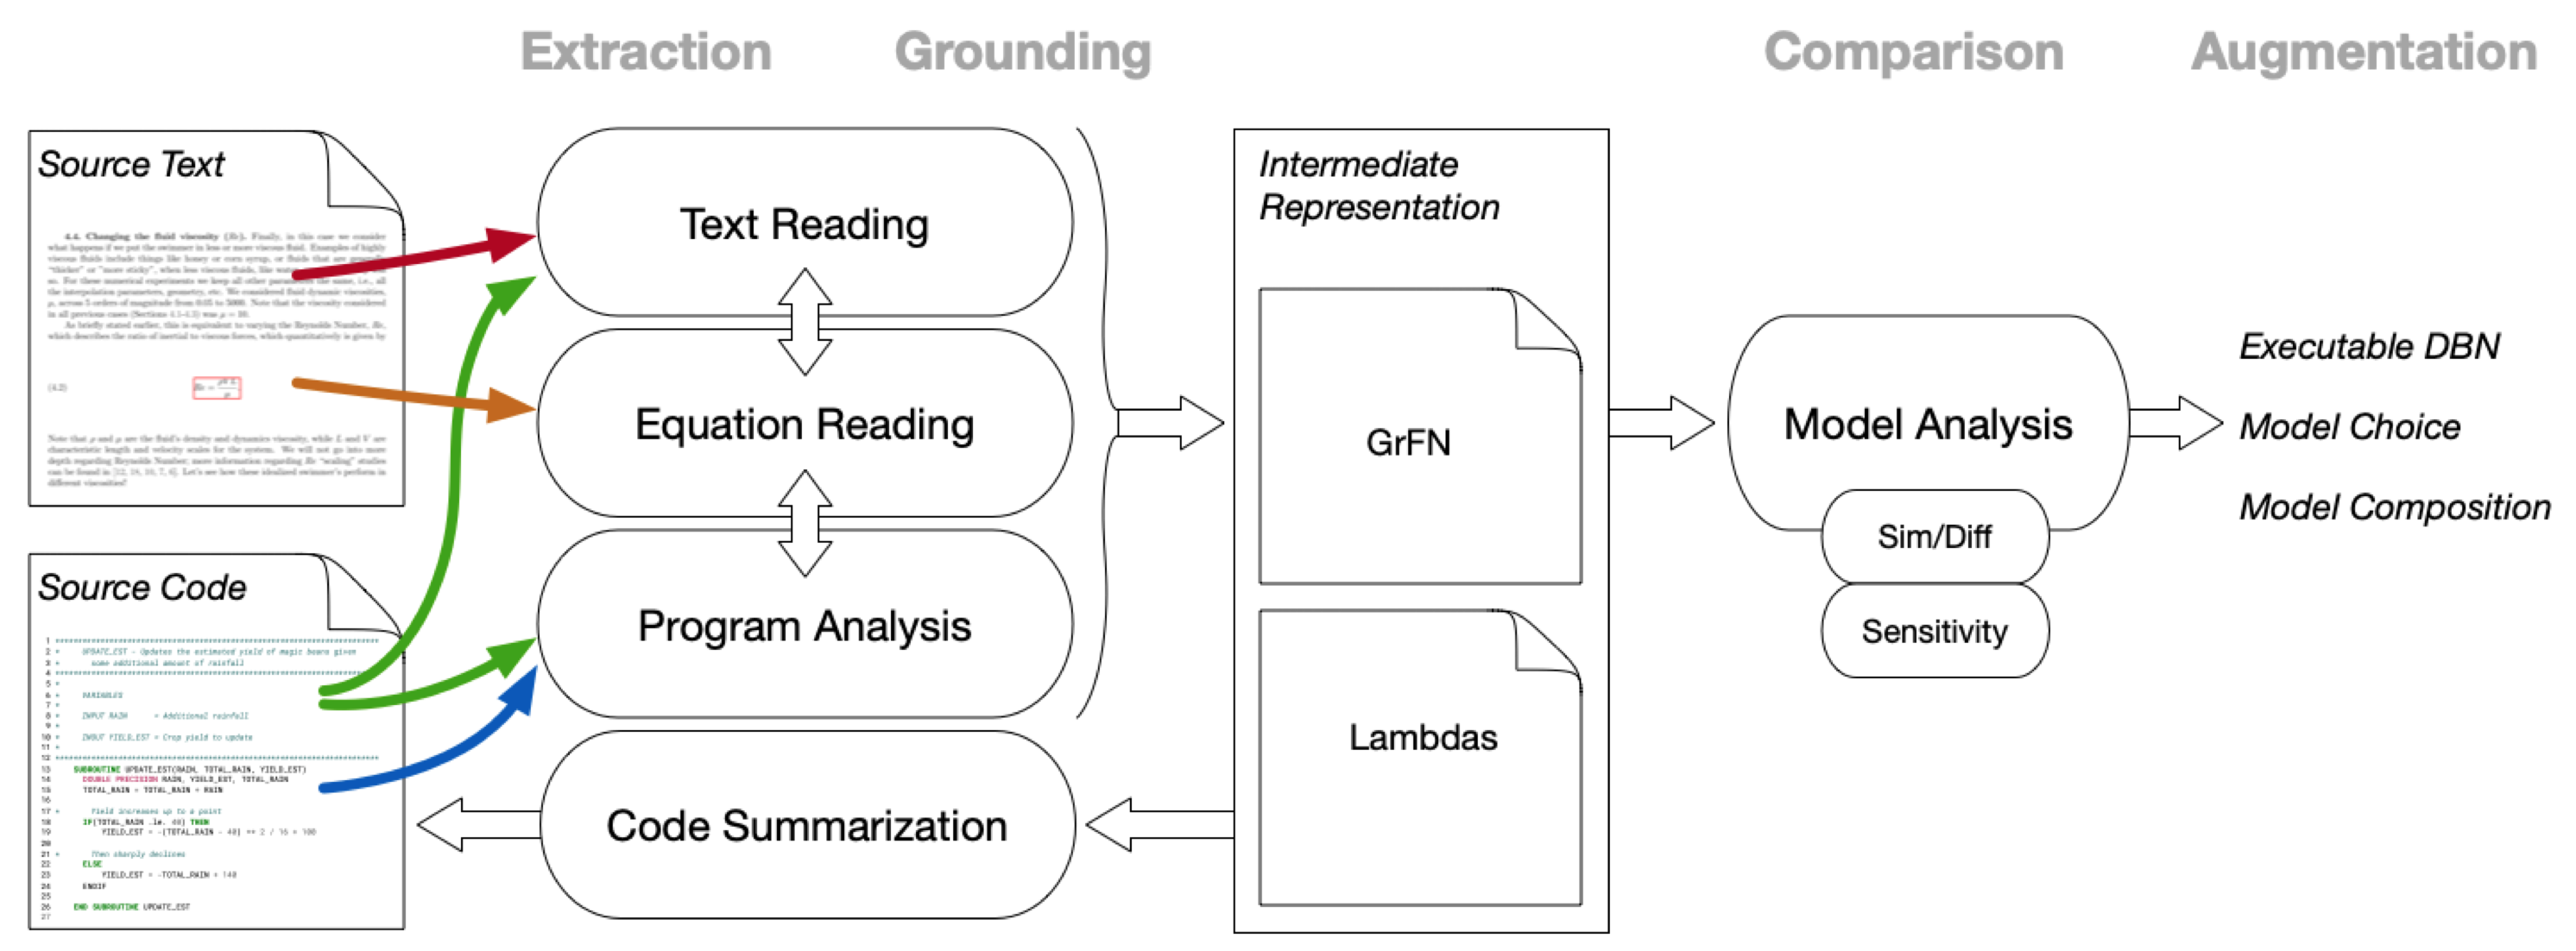
\includegraphics[width=\textwidth]{automates_pipeline}%
    \caption[The AutoMATES Pipeline]{A schematic view of the AutoMATES architecture. This figure shows the various inputs of the separate \textit{Program Analysis}, \textit{Text Reading}, and \textit{Equation Reading} modules. UMAF is contained in the portions of the pipeline comprising the intermediate representation and model analysis sections. Different colored arrows on the pipeline inputs where blue represents program source code, green represents program documentation, red represents free text found in published works, and orange represents equation images found in published works. As shown in the pipeline, the outputs from the three first modules are combined into an intermediate representation that is used by UMAF to generate models that can then be used in the model analysis phase.}
    \label{fig:automates_pipeline}
\end{figure}

Section~\ref{sec:umaf_inputs} of this chapter covers the modules of the AutoMATES architecture (Fig~\ref{fig:automates_pipeline}) that provide input to UMAF.

After discussing the inputs to UMAF, Section~\ref{sec:grfn_assembly} covers the algorithms necessary to translate a source code program to a GrFN.
In Subsection~\ref{sec:translation_func_net} we discuss how the structure of a GrFN is related to dataflow programs, and in Subsection~\ref{sec:exec_stack_creation} GrFNs are shown to be executable after the creation of a \textit{GrFN Execution Stack}.
The main purpose for transforming source code programs into GrFNs is to facilitate model analysis, and many of the model analysis methods we seek to support require probabilistic models that allow for probabilistic inference and sampling techniques to be performed on the model.
Therefore Section~\ref{sec:grfns_are_pgms} of this chapter focuses on connecting the semantics of UMAF's GrFN models to the world of probabilistic graphical modeling.
Finally, Section~\ref{sec:grfn_eval} concludes the chapter with two language feature coverage analyses that discuss the current program idiom coverage of UMAF as a means to evaluate what source code programs can be converted by UMAF into GrFN representations of models.

\section{UMAF Inputs from the AutoMATES Pipeline\label{sec:umaf_inputs}}
In this section we provide a brief overview of the current state of the modules in the AutoMATES architecture whose outputs serve as input to UMAF.
The three modules that provide inputs to UMAF are \textit{Program Analysis} (PA), \textit{Text Reading} (TR), and \textit{Equation Reading} (ER). As seen in Fig~\ref{fig:automates_pipeline}, the PA module takes a Fortran program as its input and produces an abstract syntax tree of the scientific model portion of the program as its output.
The TR module reads both associated texts from the scientific literature for a particular source code model and the documentation found in source code for that model.
From these texts the TR module extracts useful information that can be used to link the variables in source code to the scientific domain concepts represent, as they are described in text.
% The ER module module can also be used to facilitate this linking process.
The ER module uses images extracted from publications related to the source code models to reconstruct the mathematical equations present in the images.
These equations can then be linked to mathematical equations extracted from source code in order to assist in linking source code variables to descriptions of variables found in an equation that was present in a publication.
This process is especially necessary when documentation for the variables found in source code is either missing or incomplete.
In the following subsections we briefly describe the methods used by each of these modules in order to obtain the outputs required by UMAF.

\subsection{The Program Analysis Pipeline\label{sec:pa_overview}}
In order for UMAF to create a GrFN from source code it requires the source code to be transformed into a representation that captures the computations (functions) required to compute the state of variables contained in a source code program and the ``wiring'' that species how variables in the source code program are connected as inputs and outputs of the functions.
In order to fulfill both of these requests the PA module performs a translation from the original source code into two components, a \textit{function collection} that stores the computations required to compute each variable and a \textit{container collection} that records what variables are used in each program source code statement and groups them according to variable scope environments (as determined by source code idioms such as functions/subroutines, loops, conditionals, etc.).
UMAF is able to use these two components in order to produce the function network component of a GrFN that explicitly represents the wiring among variables in the GrFN while providing access to inspect the computations used to compute each variable.
An added component of the functionality of the PA module is to translate the source code programs from their initial programming language into a single intermediate representation language that can be read by UMAF.
This allows for UMAF to focus on translating a single input source (namely the statement list produced by the PA module) as opposed to needing to be able to translate all of the many programming languages and idioms into GrFN.
Currently the PA module only translates Fortran programs into the intermediate representation; however, as a component of AutoMATES the PA module is intended to translate models written in other languages and programming styles during the lifespan of the project.

The process conducted by the PA module to translate the Fortran source code for a scientific model starts by using the Open Fortran Parser (OFP) \footnote{\url{https://github.com/OpenFortranProject/open-fortran-parser}} in order to extract an abstract syntax tree (AST) \citep{aho1986dragonBook} from the original source code.
The PA module takes advantage of the AST structure to identify containers of portions of code, such as loops and function calls.
Other containers can exist in the original source code, such as unconditional branching and looping containers created by \texttt{goto} statements.
A preprocessing step in the the PA module system is to translate all unstructured containers into a structured variant that tracks input variables into the container and the output variables expected from the container.
This is necessary in order to complete the variable wiring for a GrFN across the containers found in the original source code.
Under each container exists an ordered list of statements.
Statement are either assignment statements or conditional statements, both of which produce variables that need to be wired into a GrFN and include a computation that details how the variable is produced as a product of other variables.

Assignment statements in an AST represent that a value, either a literal value or derived from a computation involving zero or more other variables, is assigned to a target variable.
The PA module identifies these forms in the AST and extracts and separate the computation as a \textit{black-box} function, associated with the variable being assigned, and adds the extracted function to the function collection.
With a minor amount of inspection, the PA module can determine what variables are used in the computation that need to be wired to the assignment variable as inputs and adds an entry to the containers statement list in the container collection.
While multiple assignment statements to the same variable can occur in a program, GrFN is concerned with the flow of data through the scientific model represented by a program.
Thus the PA module performs the additional task when translating an assignment statement of indexing updates to variables with the same name to preserve the flow of data for the wiring step of GrFN creation.
In an imperative programming language, conditional statements involve both control-flow actions and data-flow actions.
The PA module handles conditional statements by splitting the statement into a condition evaluation that regulates control flow through the conditional, and a set of decision statements, one per assignment statement found under the conditional that determines the flow of data to the variable assigned under the conditional.
The computations and wiring required for the condition and decision statements are handled similarly to the assignment statement described above and added to the function collection and statement list of the container collection respectively.
Once all containers of the original program have been processed, the function collection and container collection represent a language-agnostic view of the original source code in the form of an imperative program.
These outputs will then be sent to UMAF in order for the dataflow representation of a scientific model to be extracted from the source code.

\subsection{The Text and Equation Reading Modules \label{sec:ter_overview}}
While the PA module is able to provide all of the wiring needed to create a function network and the computations needed to make the network executable, UMAF requires additional inputs in order to perform the variable grounding necessary to create a GrFN.
These inputs come from the TR Module and the ER Module.
The information we are interested in gathering from these two modules is a mapping of variables mentioned in the program source code to real-world concepts present in the system being modeled.
In order to perform the mapping, the TR module makes use of text information from publications associated with the models, as well as variable documentation present in the source code.
The TR module first extracts possible variables from the associated publications using the ODIN\footnote{\url{https://github.com/clulab/processors/wiki/ODIN-(Open-Domain-INformer)}} event extraction framework \citep{valenzuela2015Odin}.
During the extraction process each of the variables will have a text portion associated with it that has been determined to be a description of the variable from the publication.
An example of extracting variables with associated descriptions is shown in Fig~\ref{fig:odin_extraction_example}.
The TR module can perform the mapping by computing a word-overlap score between the text description of each of the possible variables from the associated publication with the variable documentation snippets found in the source code.
Descriptions that have high enough overlap are then linked and the variables present in the source code that correspond to the documentation snippet are considered grounded to the variable extracted from the associated publication.

\begin{figure}[!htbp]
    \centering
    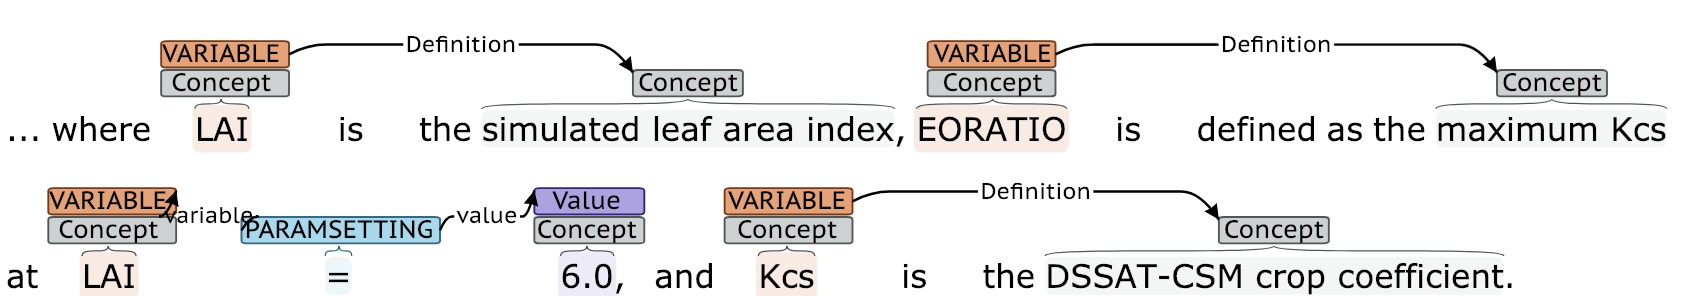
\includegraphics[width=\textwidth]{TR_Odin_extraction_rules}%
    \caption[Example Variable Extraction via ODIN]{An example of variables and associated text descriptions being extracted by the ODIN rule-based extraction framework.}
    \label{fig:odin_extraction_example}
\end{figure}

Another important source of domain concept grounding information comes from equations, which are often the best direct source of information about how different domain concepts are functionally related.
% However, sometimes documentation snippets do not exist for the variables found in source code, or the documentation could be incomplete. In these cases th
% The Equation Reading (ER) module can be used to help determine how to correctly ground variables to those found in the associated publication.
The Equation Reading (ER) module works by transforming images of equations found in the associated publication into a programmatic structure of the computation defined by the equation.
This structure can then be linked to the similar computation contained in the source code, thus linking the computation to the equation to variable definitions associated with domain concepts expressed in the surrounding text.
Once this is accomplished, the variables in the computation are linked to symbols in the initial equation.
At that point the TR module can link descriptions of variables found in the publication text to the symbols found in the equation.
With this final linking, the variables in the source code can now be transitively grounded to the descriptions of variables found in text, without ever requiring documentation about the variables to be present in the source code.
Using these two modules allows for the majority of variables present in the source code representation of a scientific model to be linked to observable phenomena, a process that we describe as \textit{grounding} the variables.
This gives UMAF the information necessary to produce GrFNs that satisfy the condition of being comparable upon the variable nodes, since variables that are \textit{grounded} to the same real-world phenomena are identified as equivalent objects across GrFNs.

\section{Constructing an Executable Grounded Function Network \label{sec:grfn_assembly}}
The goal of UMAF is to transform the information extracted by the PA, TR, and ER modules into an integrated GrFN representation.
The outline of this process is shown in Figure~\ref{fig:umaf_diagram} which details the algorithms contained in UMAF as well as an example output for each of the algorithms.
The example outputs in this figure were generated by running UMAF over the PETPT evapotranspiration model mentioned in the introduction.

\begin{figure}[!htbp]
    \centering
    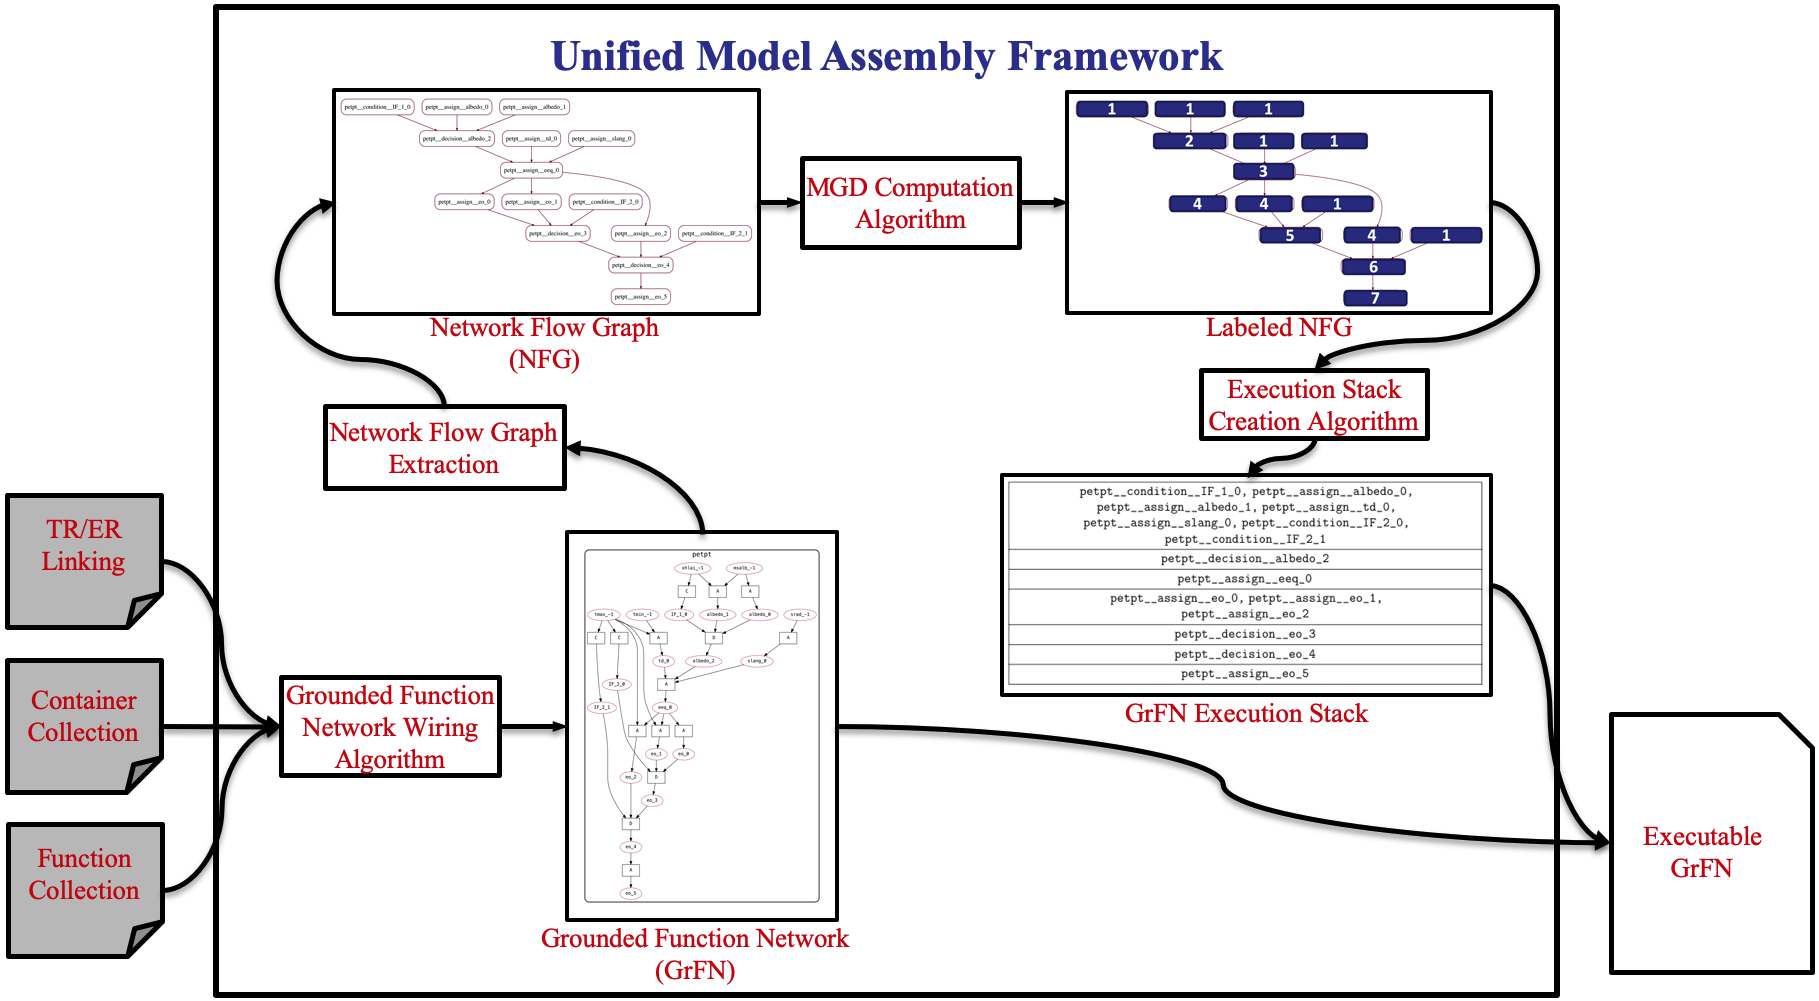
\includegraphics[width=\textwidth]{UMAF-diagram}%
    \caption[Diagram of UMAF]{This figure shows the entirety of the UMAF framework. We see that the framework takes in a function collection and a container collection from the original source code program as well as variable grounding information from associated texts. These inputs are then converted to a GrFN. Once the GrFN is constructed a Network Flow Graph is extracted from the GrFN and used to generate a GrFN Execution Stack. The GrFN and its execution stack are then combined to form the output of UMAF, an executable GrFN.}
    \label{fig:umaf_diagram}
\end{figure}

The first step of this process is to create the function network from the inputs provided by the PA module.
This process involves a translation step from the imperative representation of a program that is extracted by the PA module to a dataflow representation that can be naturally represented as a function network.
During the creation of the function network, variables contained in it can be grounded using the outputs from the TR and ER modules.
The second step required to construct a GrFN is to extract the GrFN execution stack from the function network so that the GrFN can be executed efficiently.
This section begins by detailing the processes required to translate the inputs to UMAF into a GrFN.
after discussing the translation to GrFN, we proceed to discuss the processes required to create a GrFN execution stack.
This section then concludes with a brief discussion of data type management for the data inputs of a GrFN.

\subsection{Translation to a Function Network \label{sec:translation_func_net}}
Most programs are written in languages that follow the von Neumann vision of sequential instruction execution.
This means that programs are defined as a list of instructions that are executed in the sequential order that they are written.
This representation and execution style is unnatural for a scientific model because models need not be expressed sequentially.
It is certainly the case that some computations in a scientific model must occur after others; however, there need not be a total ordering upon the computations included in the scientific model.
The only necessary restriction for executing a scientific model is that all of the inputs for a given function must populate with values before the function can be evaluated.
This execution style pairs well with programs that are written using the dataflow programming idiom \citep{johnston2004dataflowadvances}.
While traditional programming idioms, such as imperative programming, represent a program as a sequential list of instructions that are executed in a pre-defined order, dataflow programs are represented as a series of connections between inputs and outputs with connecting operations between them that function as black-box computations \citep{wadge1985lucid}.
This is the same specification as we have required for the function network component of a GrFN, and thus a GrFN is a representation of a dataflow program.
Therefore the process of creating a GrFN from the inputs provided to UMAF can be reduced to the process of translating an imperative representation of a program to a dataflow representation of a program, and then grounding the variables present in the new dataflow program.

While imperative programs are easily expressed as lines of code in flat files, this expression format is unnatural for a dataflow program.
A dataflow program, such as the GrFN created by UMAF are much more naturally expressed as graph-based data structures.
We define the underlying structure of GrFN to be a \emph{function network}.
A function network is a directed acyclic graph (DAG) \citep{bondy1976graph} that contains a set of source nodes and a set of sink nodes.
A node is considered a source node if the in-degree of the node, the number of directed edges arriving at the node, is zero.
Similarly a node is considered a sink node if the out-degree of the node, the number of directed edges leaving the node, is zero.
Function networks also contain two types of nodes, \textit{variable nodes} and \textit{function nodes}, where a variable node represents a real-world variable and a function node stores the computation necessary to compute a new variable node from a combination of other variables.
The actual graph structure is bipartite \citep{chartrand1977introGraphTheory} based on these two sets of nodes, such that no variable node has a directed edge to another variable node, and no function node has a directed edge to another function node.
Each of the variable nodes in a GrFN function network are restricted to have at-most a single incoming arc (an in-degree of one), that comes from the function node that assigns the result of a computation to that node.
Similarly a function node has only a single arc leaving the node (an out-degree of one), and this arc arrives at the variable node that is assigned the result of the function nodes container computation.
Since GrFNs are supposed to represent real-world systems, the output node set of a GrFN function network contains only variable nodes; however, the input node set of a GrFN can contain both variable and function nodes.
When representing graphical structures, plates are commonly used to represent subgraphs within the main graph.
Function networks in a GrFN also have \textit{plates}.
A plate is a function network that represents the network of variables and functions formed by an enclosed scope inside of a larger function network.
Plates in a GrFN function network can either represent single-pass or repeated execution, meaning that plates correspond with calls to subroutines and loops found in the original source code.
Above we specified that GrFNs are acyclic, meaning that the function network cannot contain any cycles.
In order to ensure this property holds and still represent loops as part of the function network, the plate for a loop implies cyclic edges upon all input variables to the loop and all created variables in the loop.
The state of looping is tracked during execution with an \textit{exit} variable, a boolean that determines when to stop looping execution for a loop plate.

The function network for a GrFN is created by performing a recursive traversal through each container in the container collection passed in to UMAF by the PA module.
Algorithm~\ref{alg:func_net_wiring}, shown below, generates a function network to serve as the basis for a GrFN.

\FloatBarrier
\begin{algorithm}
  \caption{GrFN Wiring Algorithm}
  \label{alg:func_net_wiring}
  \begin{algorithmic}[1]
    \Procedure{WireNetwork}{$\mathcal{C},~\mathcal{F}$} \Comment{Creates a GrFN}
    \State $root \gets \Call{getRootContainer}{\mathcal{C}}$
    \State $N \gets$ \Call{WireContainer}{$root,~\mathcal{C},~\mathcal{F}$}
    \State \Return $N$
    \EndProcedure

    \Procedure{WireContainer}{$C,~\mathcal{C},~\mathcal{F}$} \Comment{Creates a function network}
      \State $N \gets (V,~E,~P)$
      \ForAll{$s \in C.statements$} \Comment{Process the containers statements}
        \If{$\Call{type}{s} = call$} \Comment{Perform wiring for container $s$}
          \State $C^{'} \gets \Call{getContainerFrom}{s.name,~\mathcal{C}}$
          \State $N^{'} \gets$ \Call{WireContainer}{$C^{'},~\mathcal{C},~\mathcal{F}$}
          \State $N^{'}.inputs \gets \{ v \mid v \in N.V ~\land~ v \in s.inputs \}$
          \ForAll{$(i,~o) \in N^{'}.inputs, N^{'}.outputs$}
            \State \Call{push}{$o,~N.V$}
            \State \Call{push}{$(i,~o),~N.E$}
          \EndFor
          \State \Call{push}{$N^{'},~N.P$}
        \Else \Comment{Wire inputs and outputs for statement $s$}
          \State $fn \gets \mathcal{F}(s.name)$
          \State \Call{push}{$s.output,~N.V$}
          \State \Call{push}{$fn,~N.V$}
          \State \Call{push}{$(fn,~s.output),~N.E$}
          \ForAll{$i \in s.inputs$}
            \State \Call{push}{$i,~N.V$}
            \State \Call{push}{$(i,~fn),~N.E$}
          \EndFor
        \EndIf
      \EndFor
      \State \Return $N$
    \EndProcedure
  \end{algorithmic}
\end{algorithm}
\FloatBarrier

The algorithm involves wiring all statements found in each container of the container collection during the recursive traversal of the containers.
For each container a new function network, $N$, is defined as a tuple $(V,~E,~P)$ where $V$ is the set of vertices in the network, $E$ is the set of edges in the network, and $P$ is the set of plates (or subnetworks) contained in the network $N$.
Each statement in the container with its corresponding computation from the function collection is wired with its inputs and outputs as edges into $E$ and the nodes used to store the variables and computation are added into $V$.
Once a new function network has been completely wired from a container it is added to the plate set $P$ for its parent function network.
This process continues until all containers have been wired into function networks that form a function network for the overall model.
Figure~\ref{fig:statement_wiring} illustrates examples of the GrFN wiring for statements that can be found in Fortran source code, as well as how plates are represented in a GrFN in correspondence to enclosed scopes found in the original source code.

\FloatBarrier
\begin{figure}[!htbp]
  \centering
  \subfloat[Assignment Statement Wiring]{
    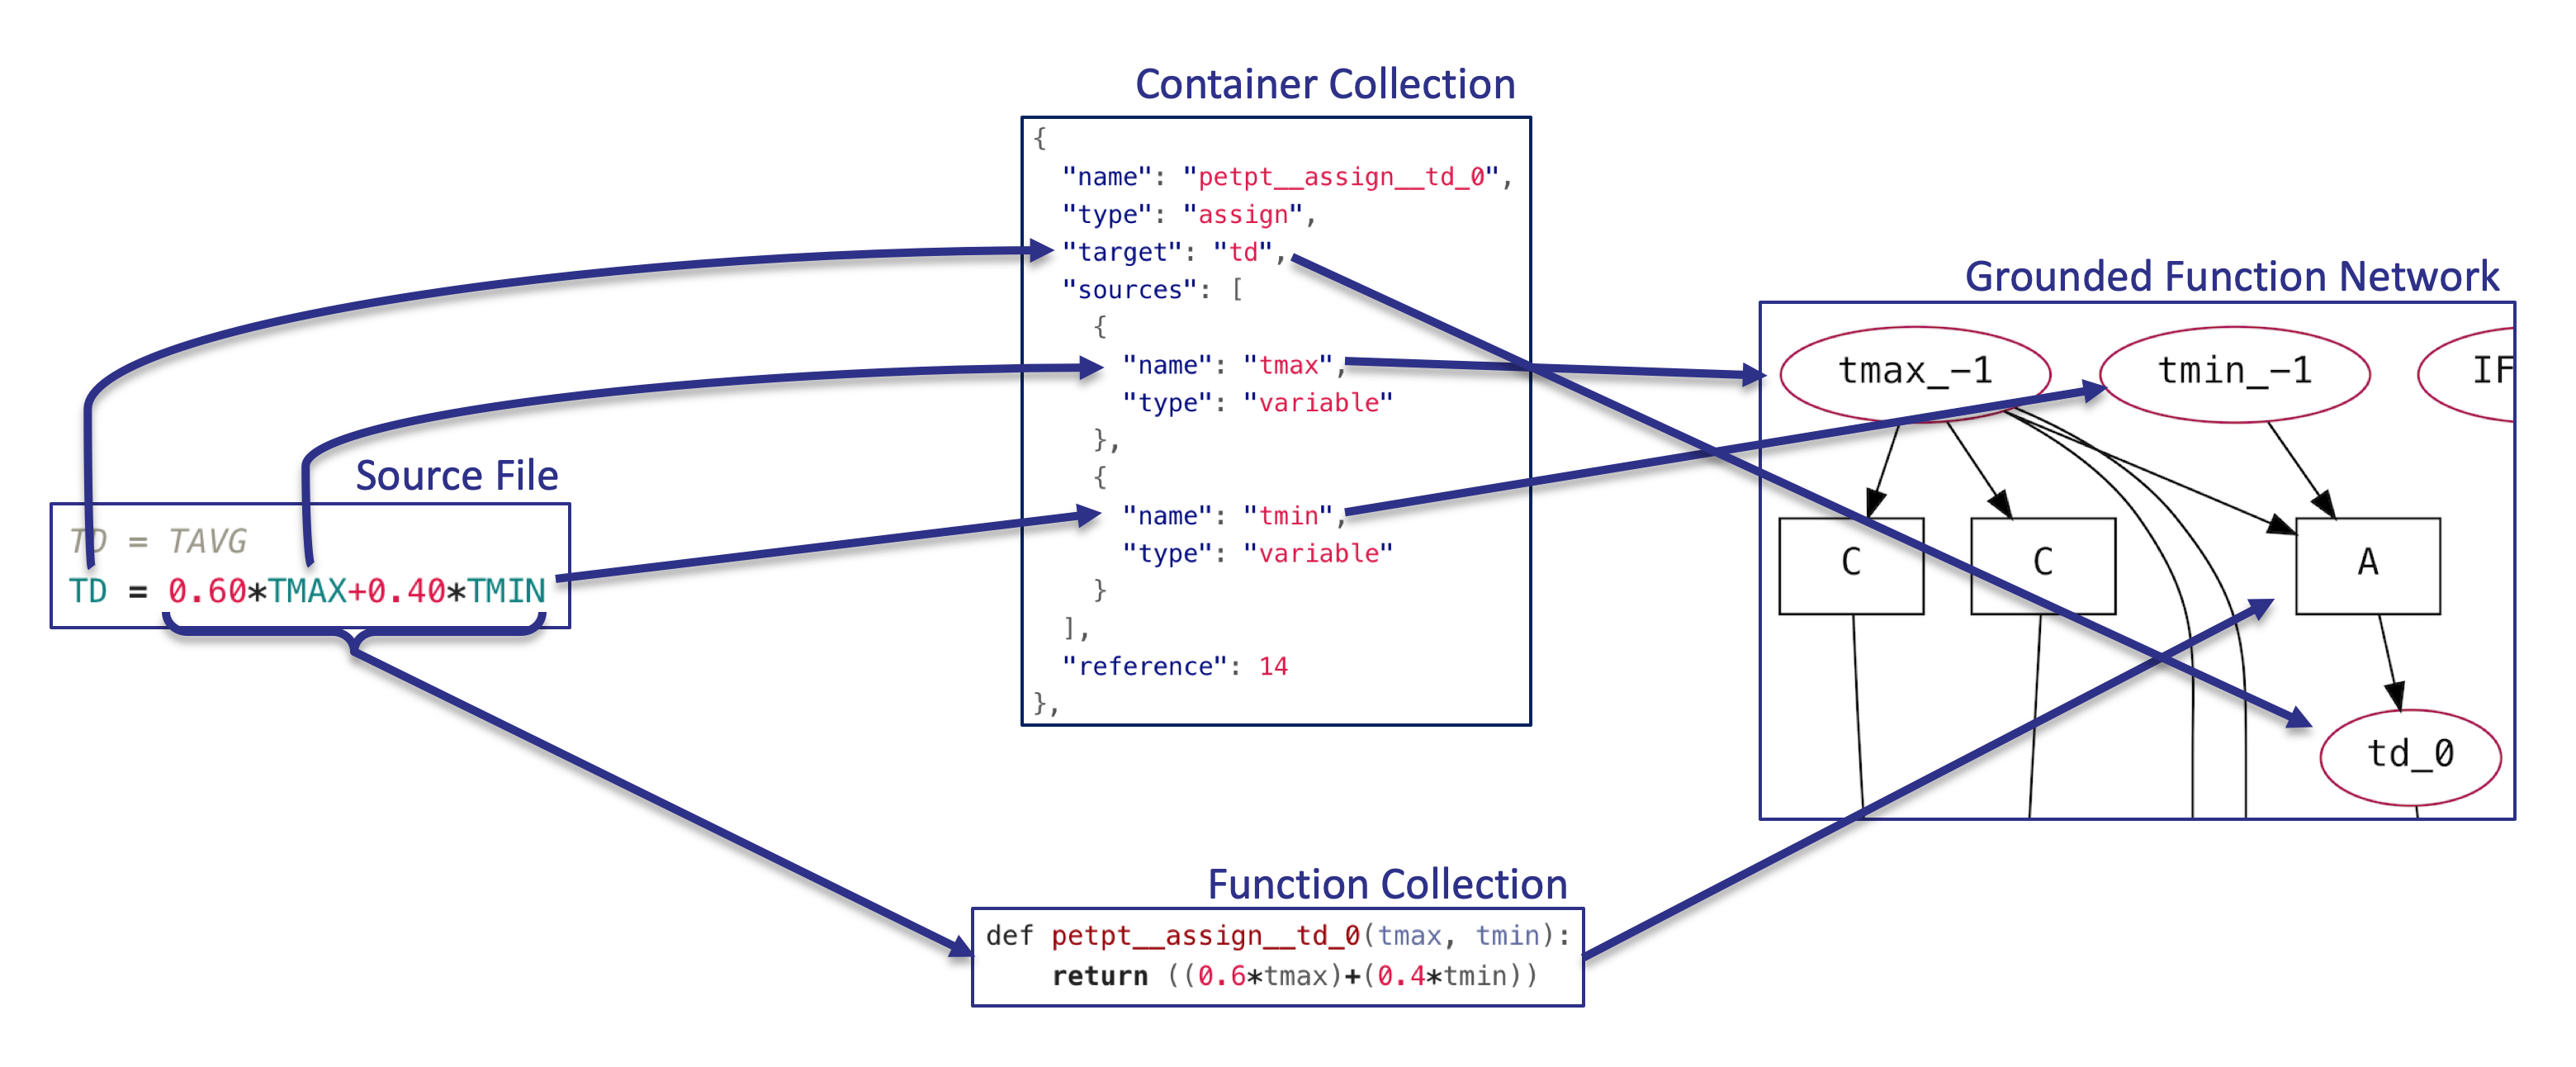
\includegraphics[width=.75\textwidth]{assg-wiring}
  }\\
  \subfloat[Conditional Statement Wiring]{
    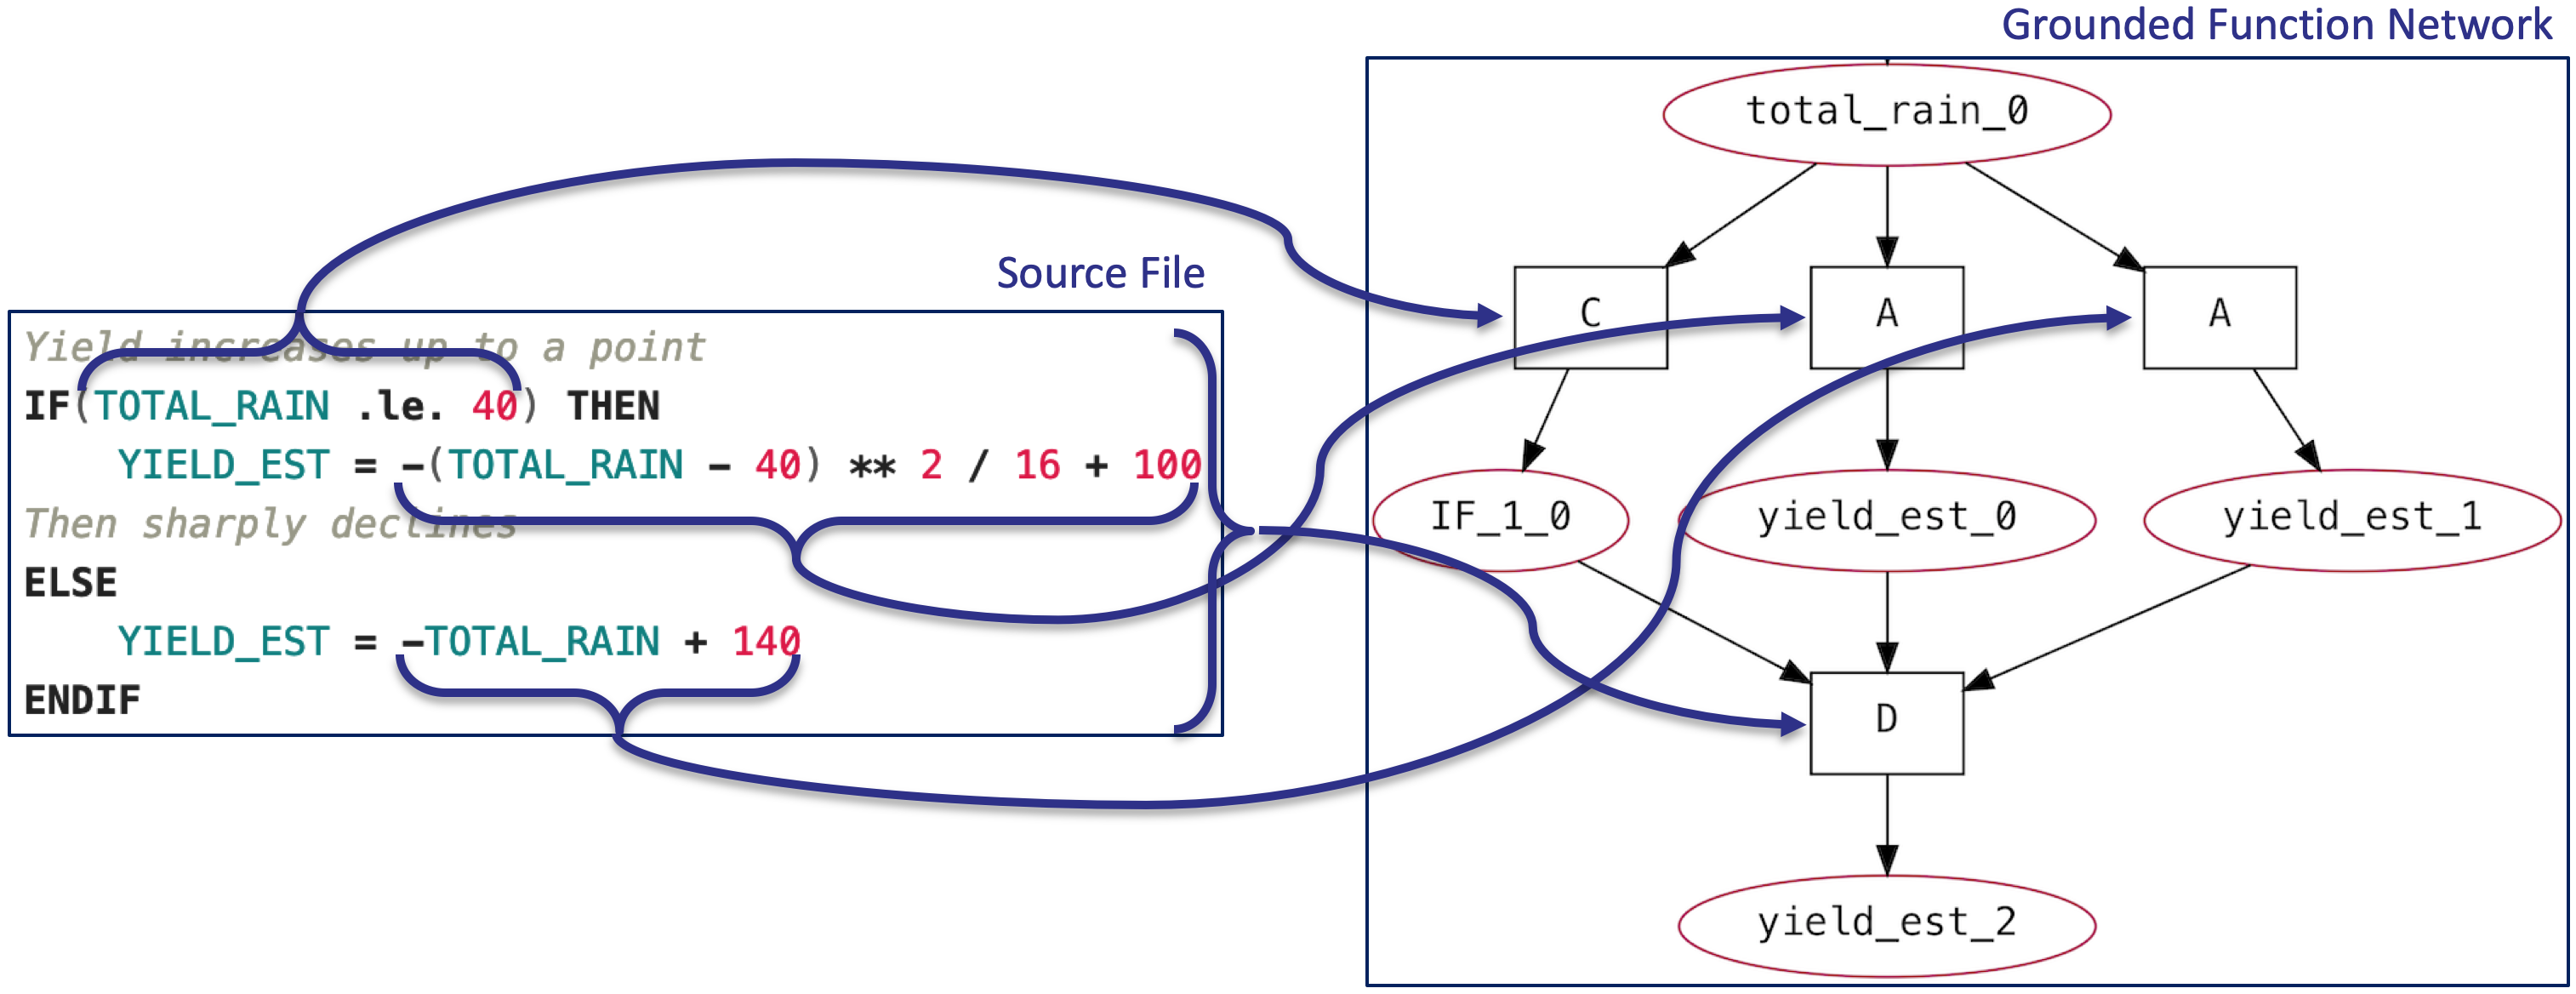
\includegraphics[width=.75\textwidth]{conditional-wiring}
  }\\
  \subfloat[Container Plate Wiring]{
    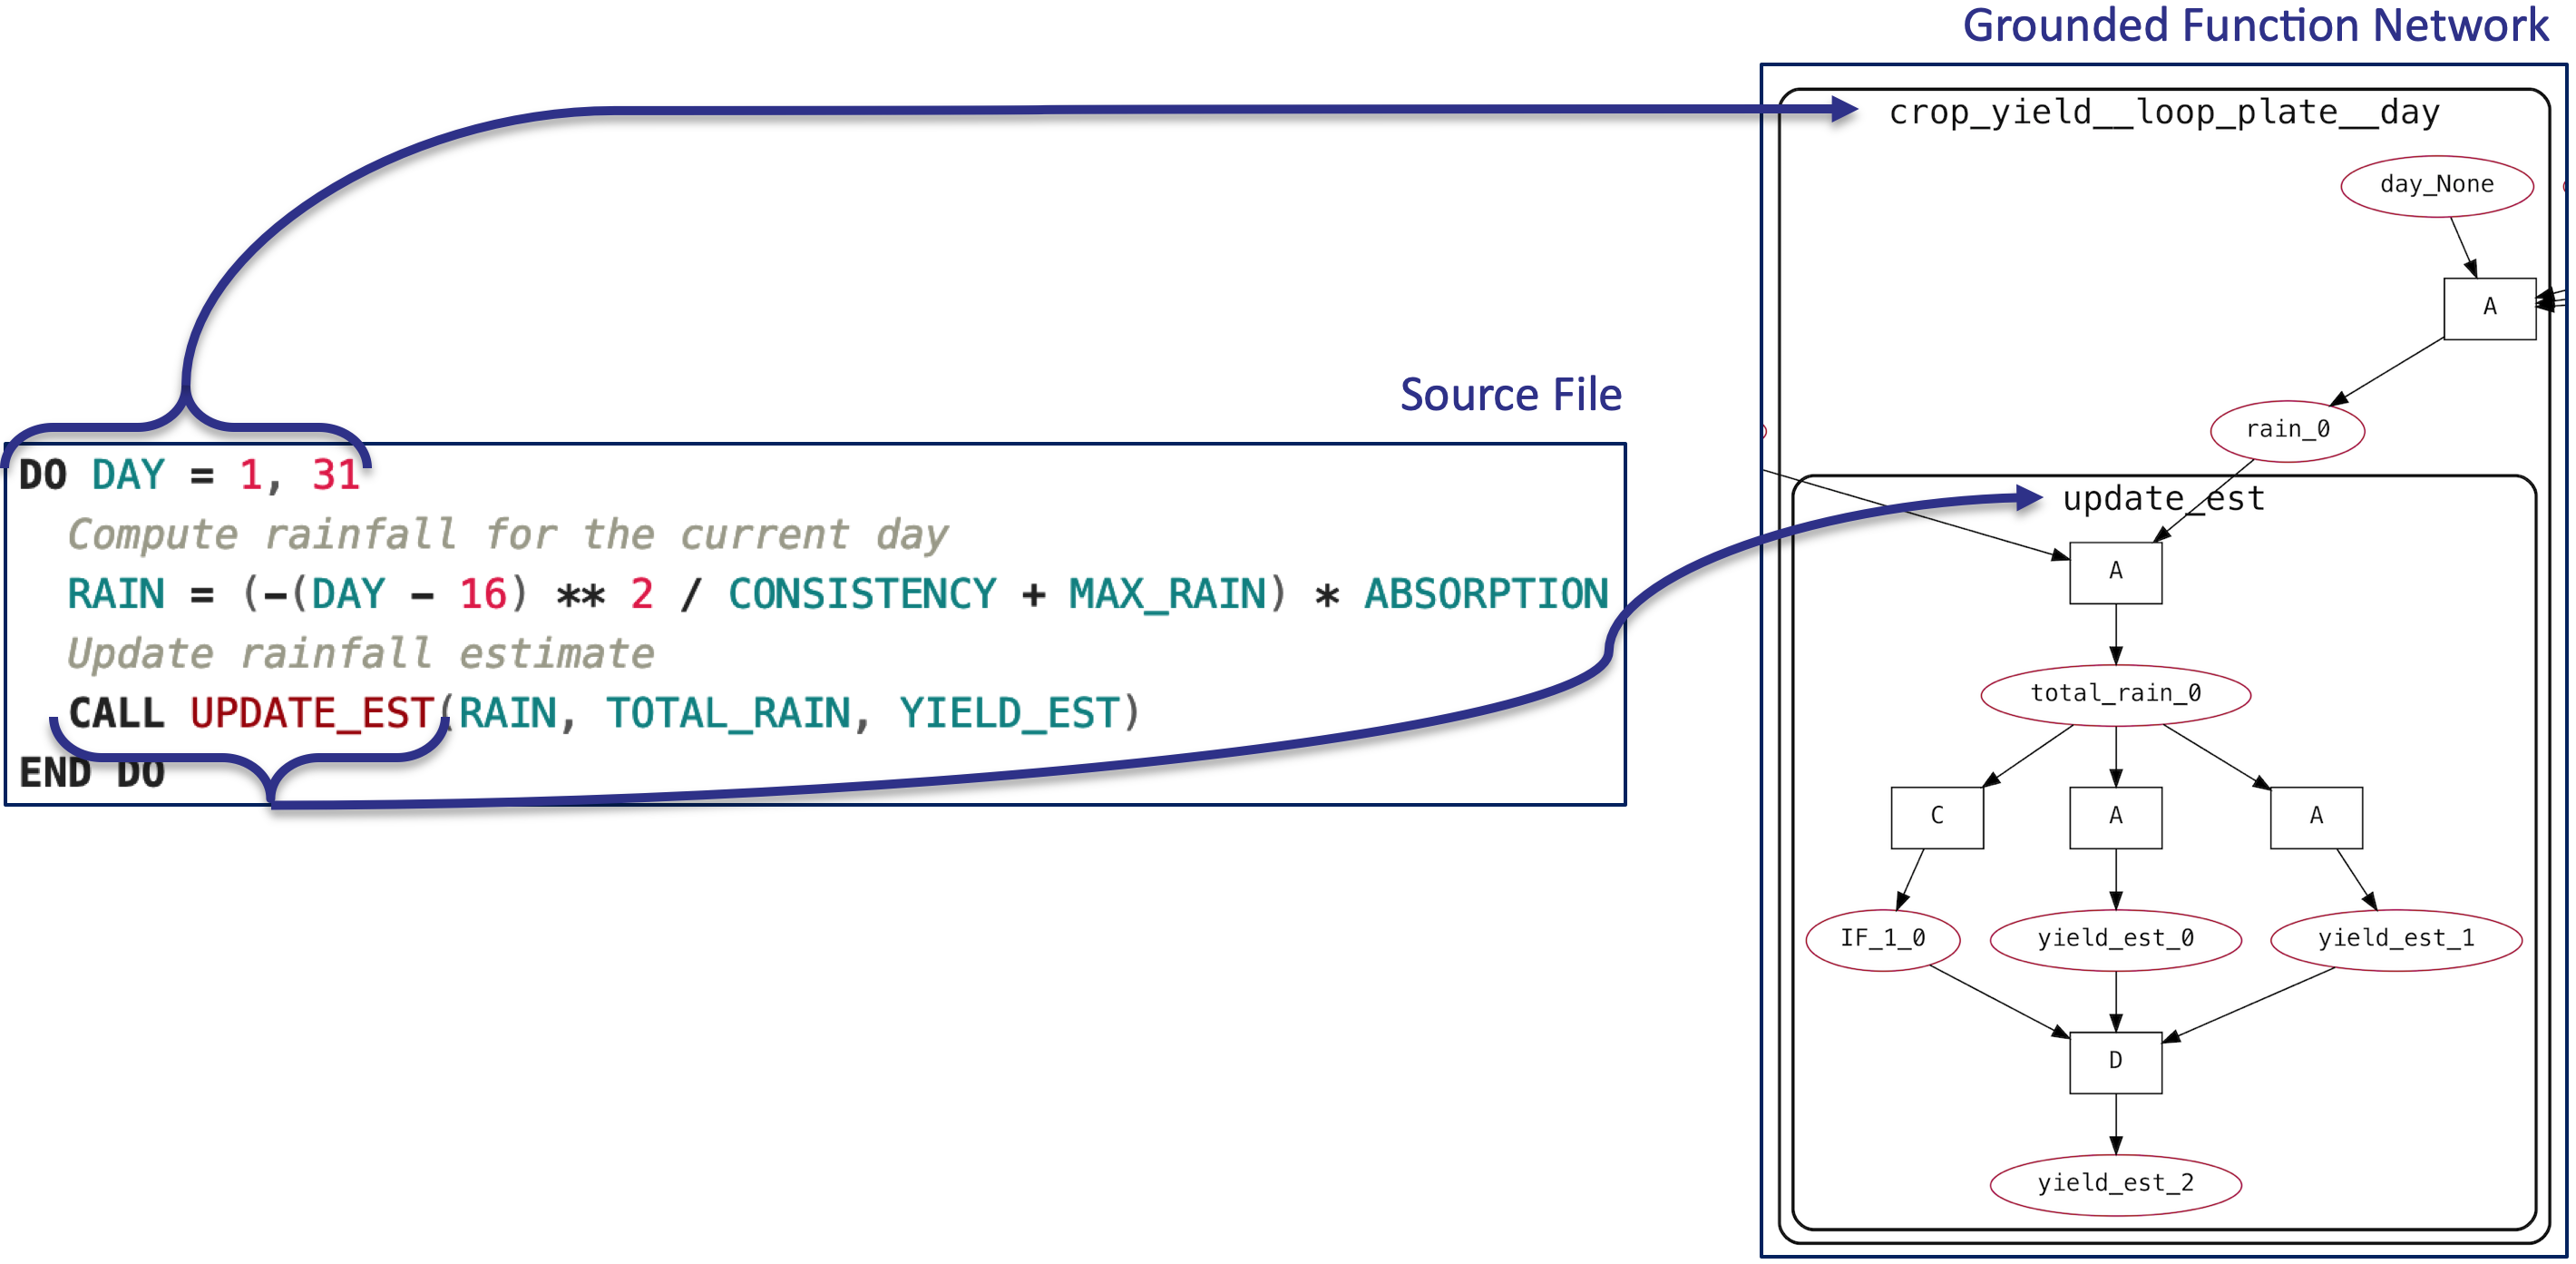
\includegraphics[width=.75\textwidth]{container-wiring}
  }
  \caption[Source Code to GrFN Wiring Examples]{Examples of the GrFN wiring for simple assignment statements, conditional statements, and nested scopes found in Fortran source code. The simple assignment statement example also details how the information found in source code is expressed in the container/function collections and then translated into a GrFN.}
  \label{fig:statement_wiring}
\end{figure}
\FloatBarrier

The only additional processing left to create a GrFN is to complete a traversal of the function network in order to visit every variable node, and to ground the variable nodes that have been linked using the inputs from the TR and ER modules.
Once the traversal is complete the translation to GrFN has been completed.
Figure~\ref{fig:grfn_cgs} shows two completed GrFNs one for the ASCE model and one for the Priestley Taylor model of potential evapotranspiration.
These GrFNs were translated from the actual Fortran source code for these two models from the DSSAT code base, both of which are available in Appendix~\ref{appendix:a}.
The visual representations of GrFNs include the variables, represented as circle nodes, with names derived from the names extracted in the source code and variable name grounding inference; the variable names also include a numeric index representing variable state changes during processing (see text for further details).
Function nodes are depicted as squares with a single letter representing the type of function contained at the node.
Function types include: assignment (A), conditional (C), decision (D), or literal (L).

\FloatBarrier
\begin{figure}[!htbp]
  \centering
  \subfloat[PETPT GrFN]{
    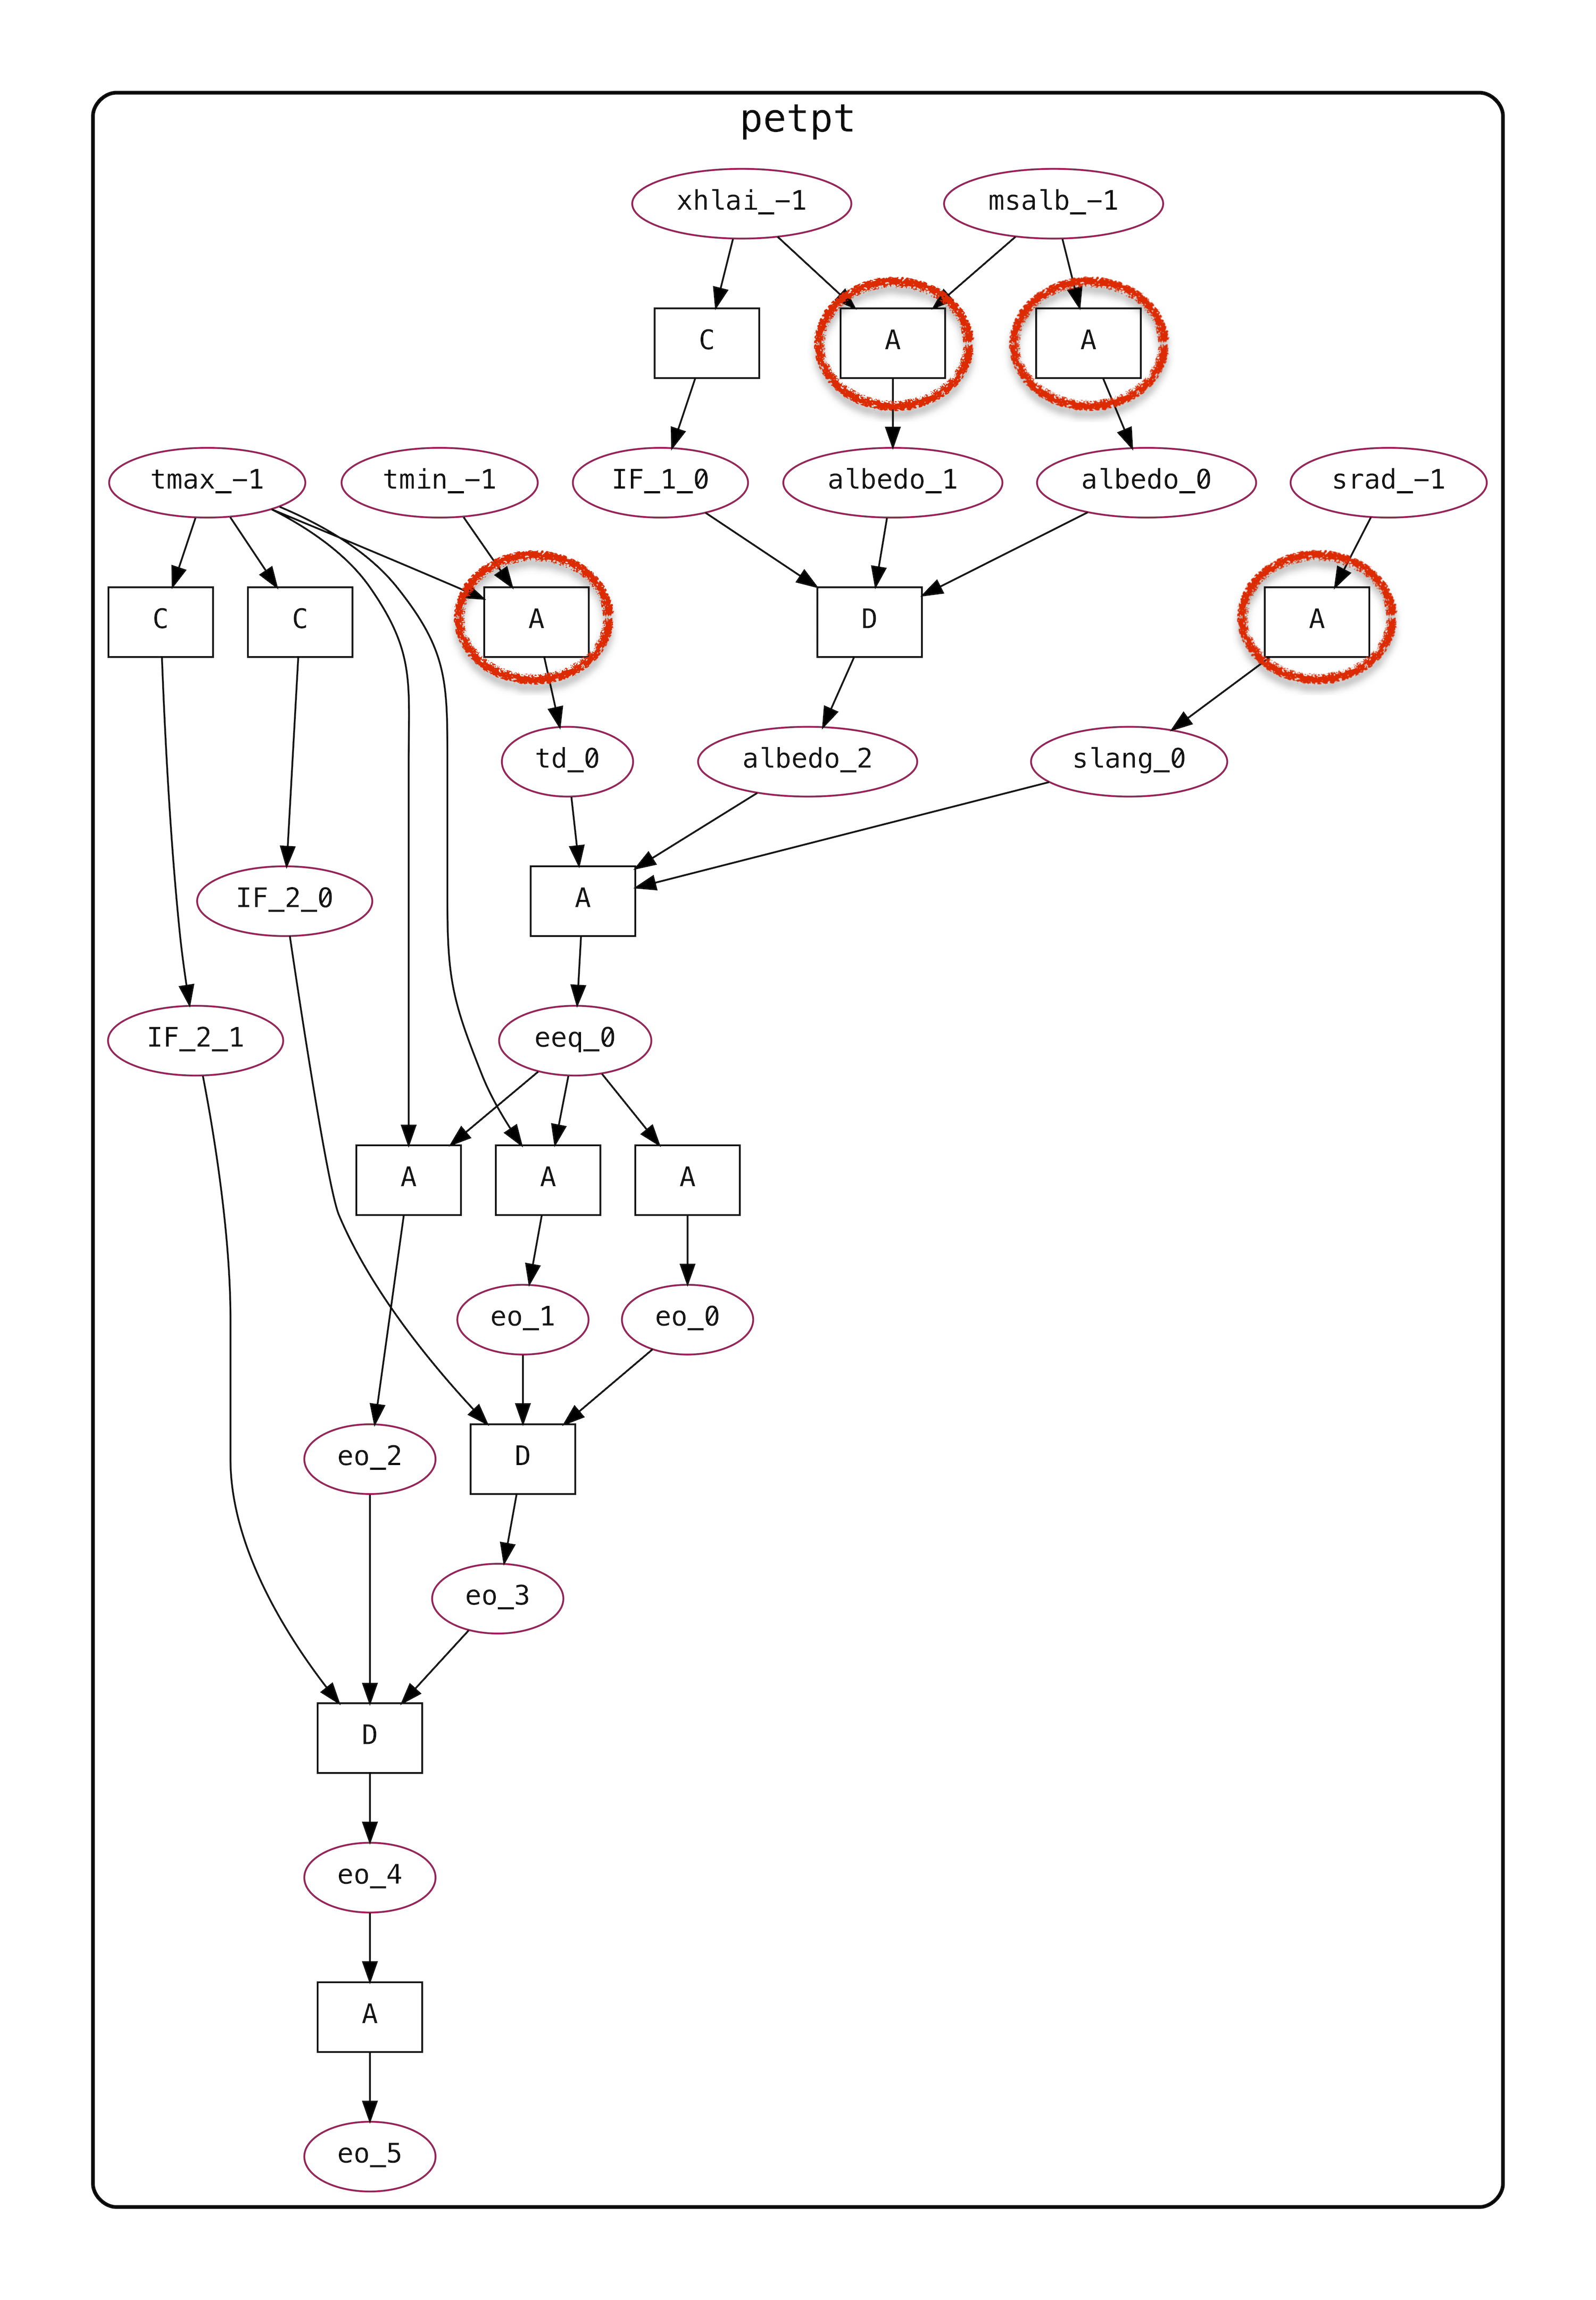
\includegraphics[width=0.48\textwidth]{PETPT_GrFN_smaller}
  }
  \hfill
  \subfloat[PETASCE GrFN]{
    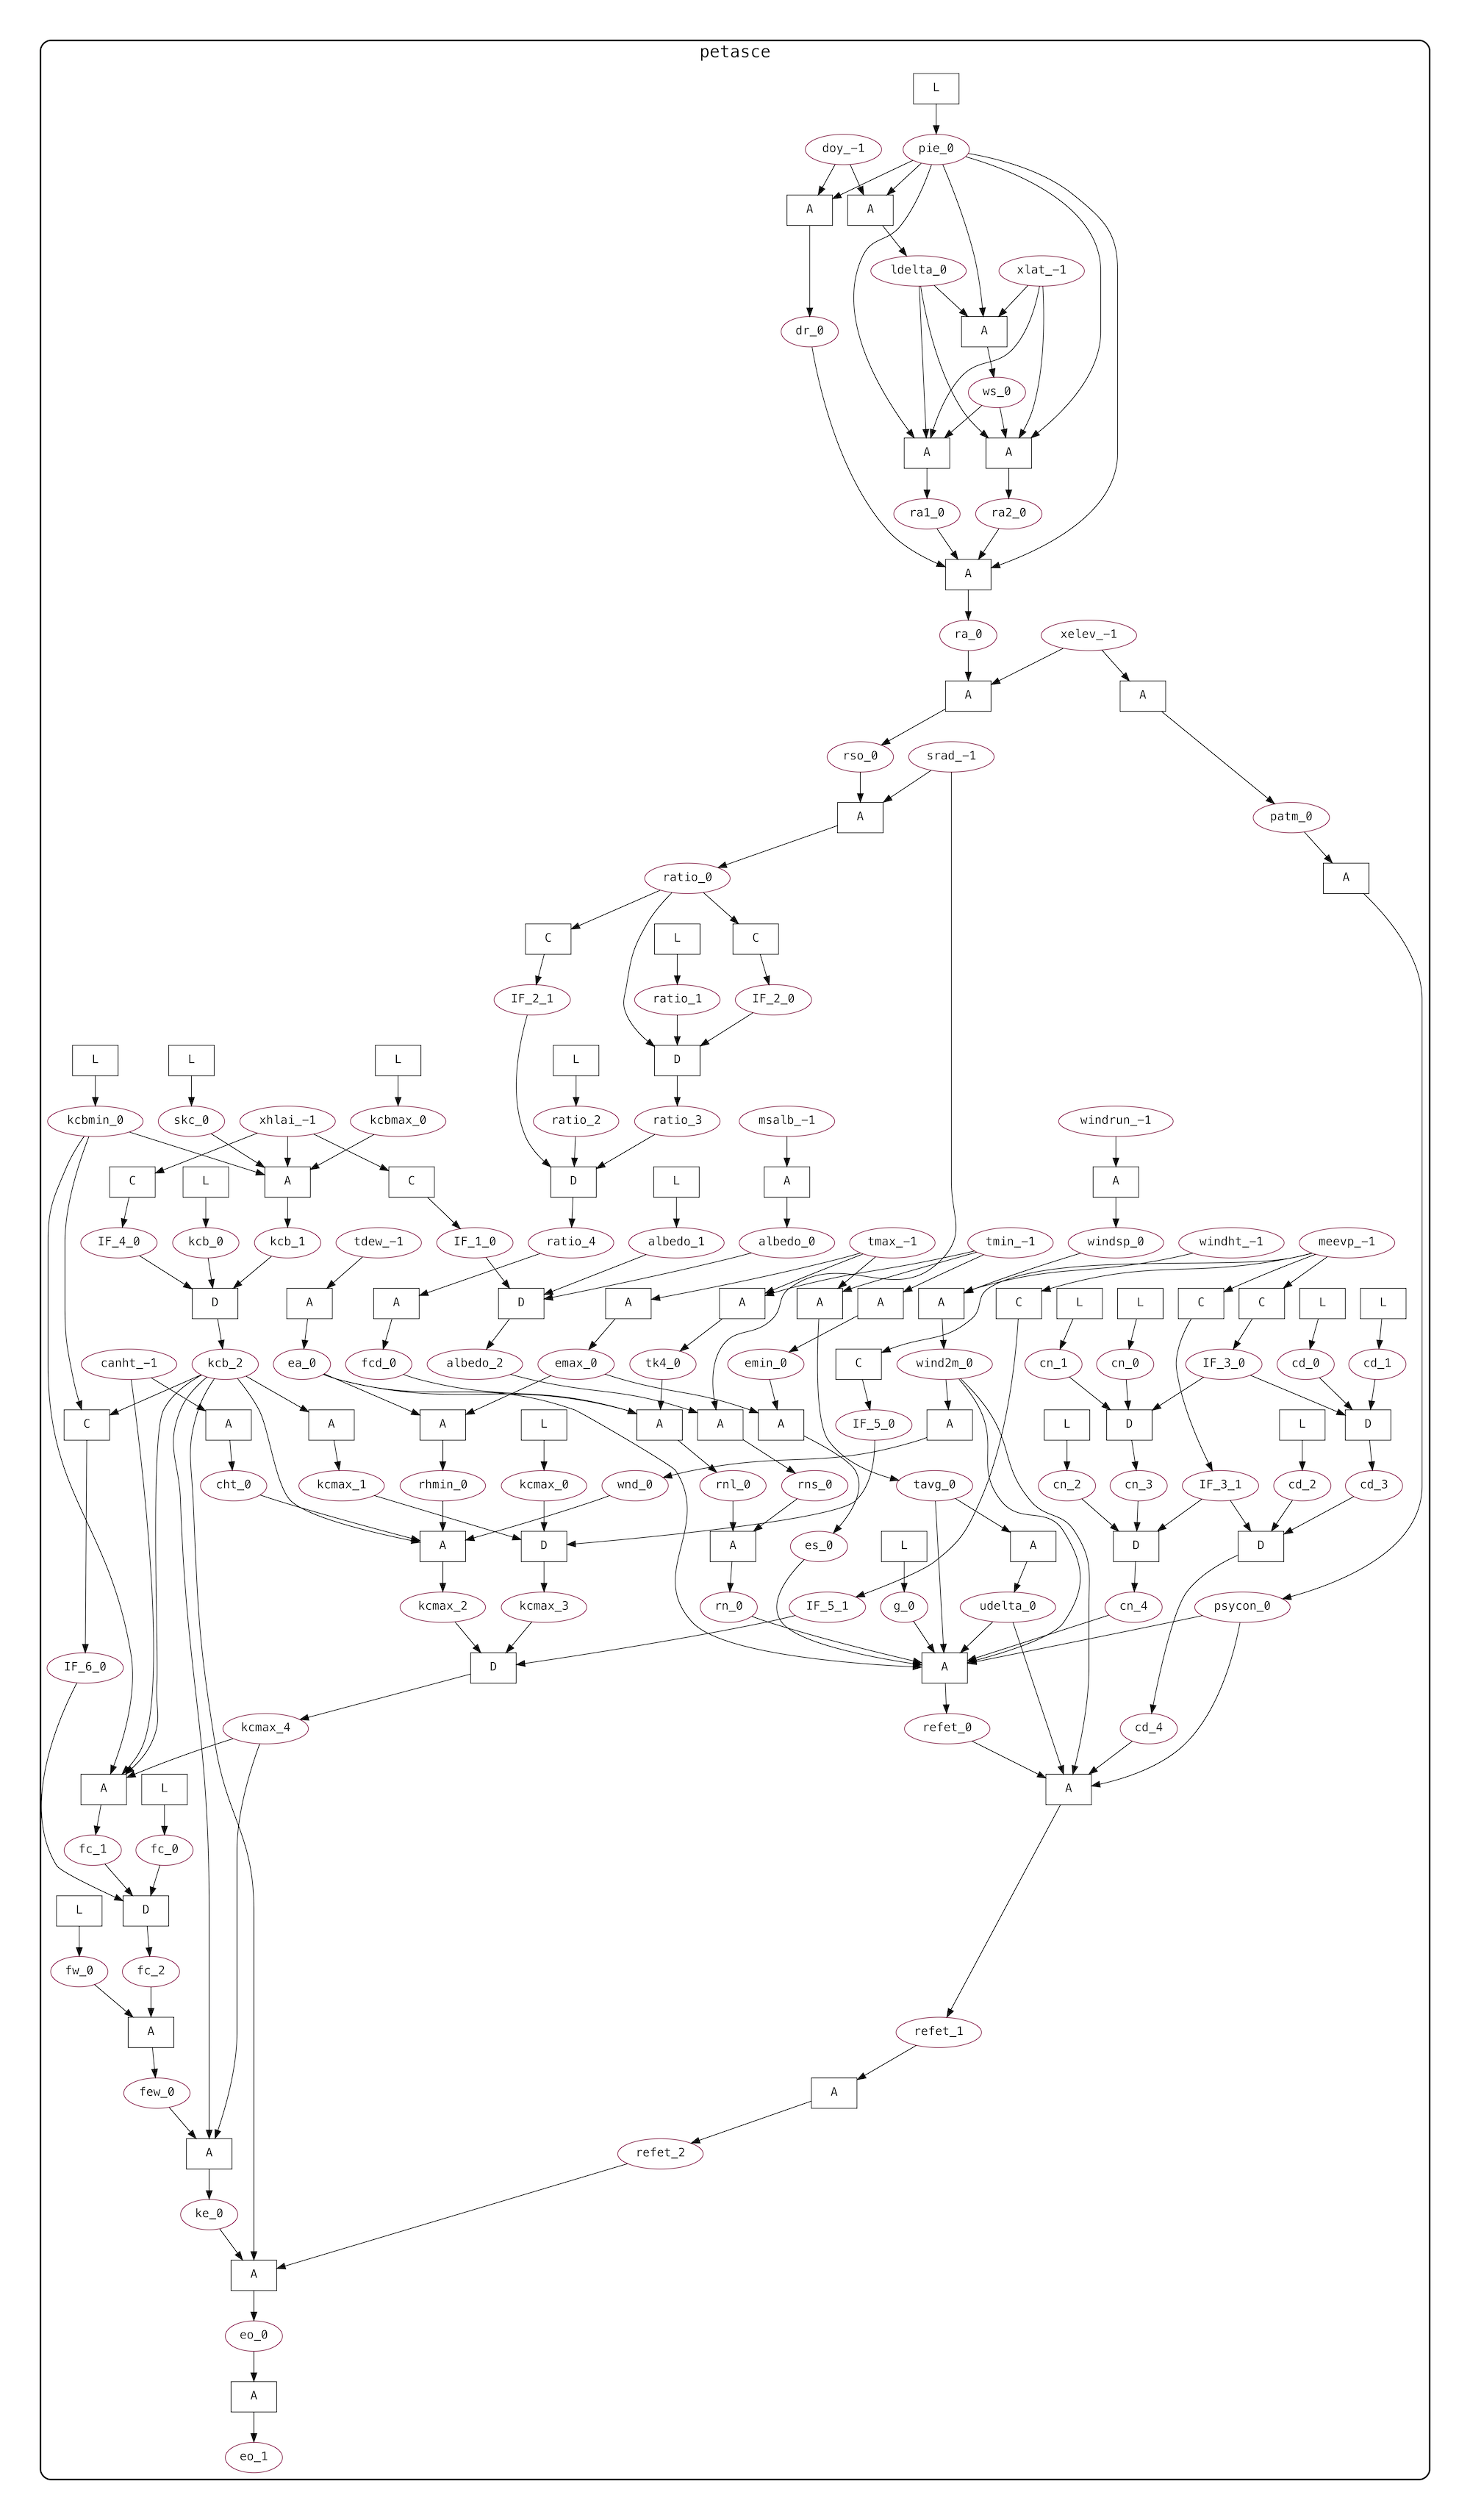
\includegraphics[width=0.48\textwidth]{PETASCE_GrFN_smaller}
  }
  \caption[Evapo-transpiration GrFN Examples]{GrFNs for the PETPT and PETASCE evapotranspiration modules.}
  \label{fig:grfn_cgs}
\end{figure}
\FloatBarrier

\subsection{Creating a GrFN Execution Stack \label{sec:exec_stack_creation}}
Creating a GrFN allows us to formally represent a scientific model from source code as a dataflow program.
However, if we wish to analyze the GrFN, then we need the ability to execute GrFNs given a set of input values.
A GrFN can be executed by executing the lambda functions stored in all of the function nodes.
As stated in the previous subsection, the function nodes rely upon having values populated at each of their input variable nodes in order to execute their lambda functions.
Therefore, if an ordering is defined over the execution of the function nodes contained in a GrFN ensures that no function node is executed before values populate to the node, then the GrFN is able to execute correctly.

A Naïve first-pass solution to accomplish this goal would be to use a graph traversal from the output to the inputs where at each function node, the node determines whether values for each input variable node have been populated.
For any input variable nodes that have not been populated, the function node calls the parent function node responsible for computing the value of the input variable node.
Once all such calls have returned, the original function is evaluated. This recursive calling procedure is very similar to message-passing, a method for inference on factor graphs \citep{bishop2006pattern}.
While this would ensure correct model execution, this method of handling execution is not as efficient as possible.
Two obvious inefficiencies are that the recursive call structure requires additional function setup and calls to the execution, on the order of the number of functions included in the computation graph, and this execution style requires recursive message passing for each execution.

These two concerns can be addressed by creating an execution stack comprised of all the function nodes contained in the GrFN.
A normal execution stack would be a sequential ordering of execution of all the nodes, where each item in the stack is a single function to execute.
Since GrFN is a dataflow program, we can relax this requirement to have execution levels in the execution stack.
Each execution level includes a list of functions that can be computed in any order.
This implies that the execution stack is equivalent to a partially ordered set (poset) \citep{simovici2008miningTools} upon the function nodes.
Higher levels in the stack need to be executed before lower levels, and when constructed properly each level of the stack should contain only the functions that need to be executed before moving to the next execution layer.
Computing over a GrFN using this execution stack ensures that we still see the benefits of parallel execution when possible, but also have the least amount of setup and additional function calls necessary for successive rounds of execution.

Creating the execution stack requires a series of separate computations.
First a network flow graph (NFG) \citep{allen1970CFG} must be extracted from the GrFN.
A GrFN is bipartite \citep{bondy1976graph} with respect to the variable and function nodes, such that no variable node is adjacent to another variable node and vice-versa for a function node.
Therefore a GrFN NFG can be extracted from a GrFN by simply squashing any variable node between a pair of function nodes into a singular edge connecting the two function nodes.
The nodes in a GrFN NFG represent function nodes in the actual GrFN and connections between nodes represent the flow of data through the function nodes in the GrFN.

\FloatBarrier
\begin{figure}[!htbp]
    \centering
    \includegraphics[width=\columnwidth]{PETPT_GrFN_NFG}%
    \caption[PETPT GrFN Network Flow Graph]{A visualization of the Network Flow Graph (NFG) for the PETPT model.}
    \label{fig:petpt_nfg}
\end{figure}
\FloatBarrier

Now that we have an NFG we must find the maximum graph distance (MGD) from an input node to every internal and output node in the NFG.
Graph distance is defined as the number of directed arcs that must be traversed to go from a source node to a destination node.
Using this metric ensures that any function node, $f$, is placed in a deep enough execution level to ensure that all prerequisite functions have executed before attempting execution of $f$.
UMAF computes the MGD for each node in a GrFN NFG using Algorithm~\ref{alg:mgd_algorithm} shown below, which computes the MGDs by walking over the nodes in the NFG, starting from the inputs and labeling nodes according to the number of arcs traversed during the path to the node from that input.

\FloatBarrier
\begin{algorithm}
  \caption{Maximum Graph Distance Computation}
  \label{alg:mgd_algorithm}
  \begin{algorithmic}[1]
    \Procedure{MGD}{$F$} \Comment{F is a GrFN Network Flow Graph}
      \State $N \gets \{n \mid n \in F.V~\land~\Call{isInputNode}{n, F} \}$ \Comment{Initialize $N$ from $F$}
      \State $d \gets 1$
      \While{$N \neq \emptyset$}
        \ForAll{$n \in N$}
          \State $n.dist \gets d$ \Comment{Mark nodes with current distance}
        \EndFor
      	\State $N \gets \left\{ c \mid c \in \bigcup\limits_{n~\in~N}^{} \Call{isSuccessorOf}{c, n} \right\}$ \Comment{Collect successors of $N$}
        \State $d \gets d + 1$
      \EndWhile
      \State \Return $d$
    \EndProcedure
  \end{algorithmic}
\end{algorithm}

Once the MGD for each node in the NFG has been computed, the nodes in the NFG will then be labeled with their MGD values.
Figure~\ref{fig:labeled_petpt_nfg} shows the labeled nodes for the PETPT NFG that was introduced in Figure~\ref{fig:petpt_nfg}.
The MGDs can be used to place nodes of the NFG into execution stack levels.

\begin{figure}[!htbp]
    \centering
    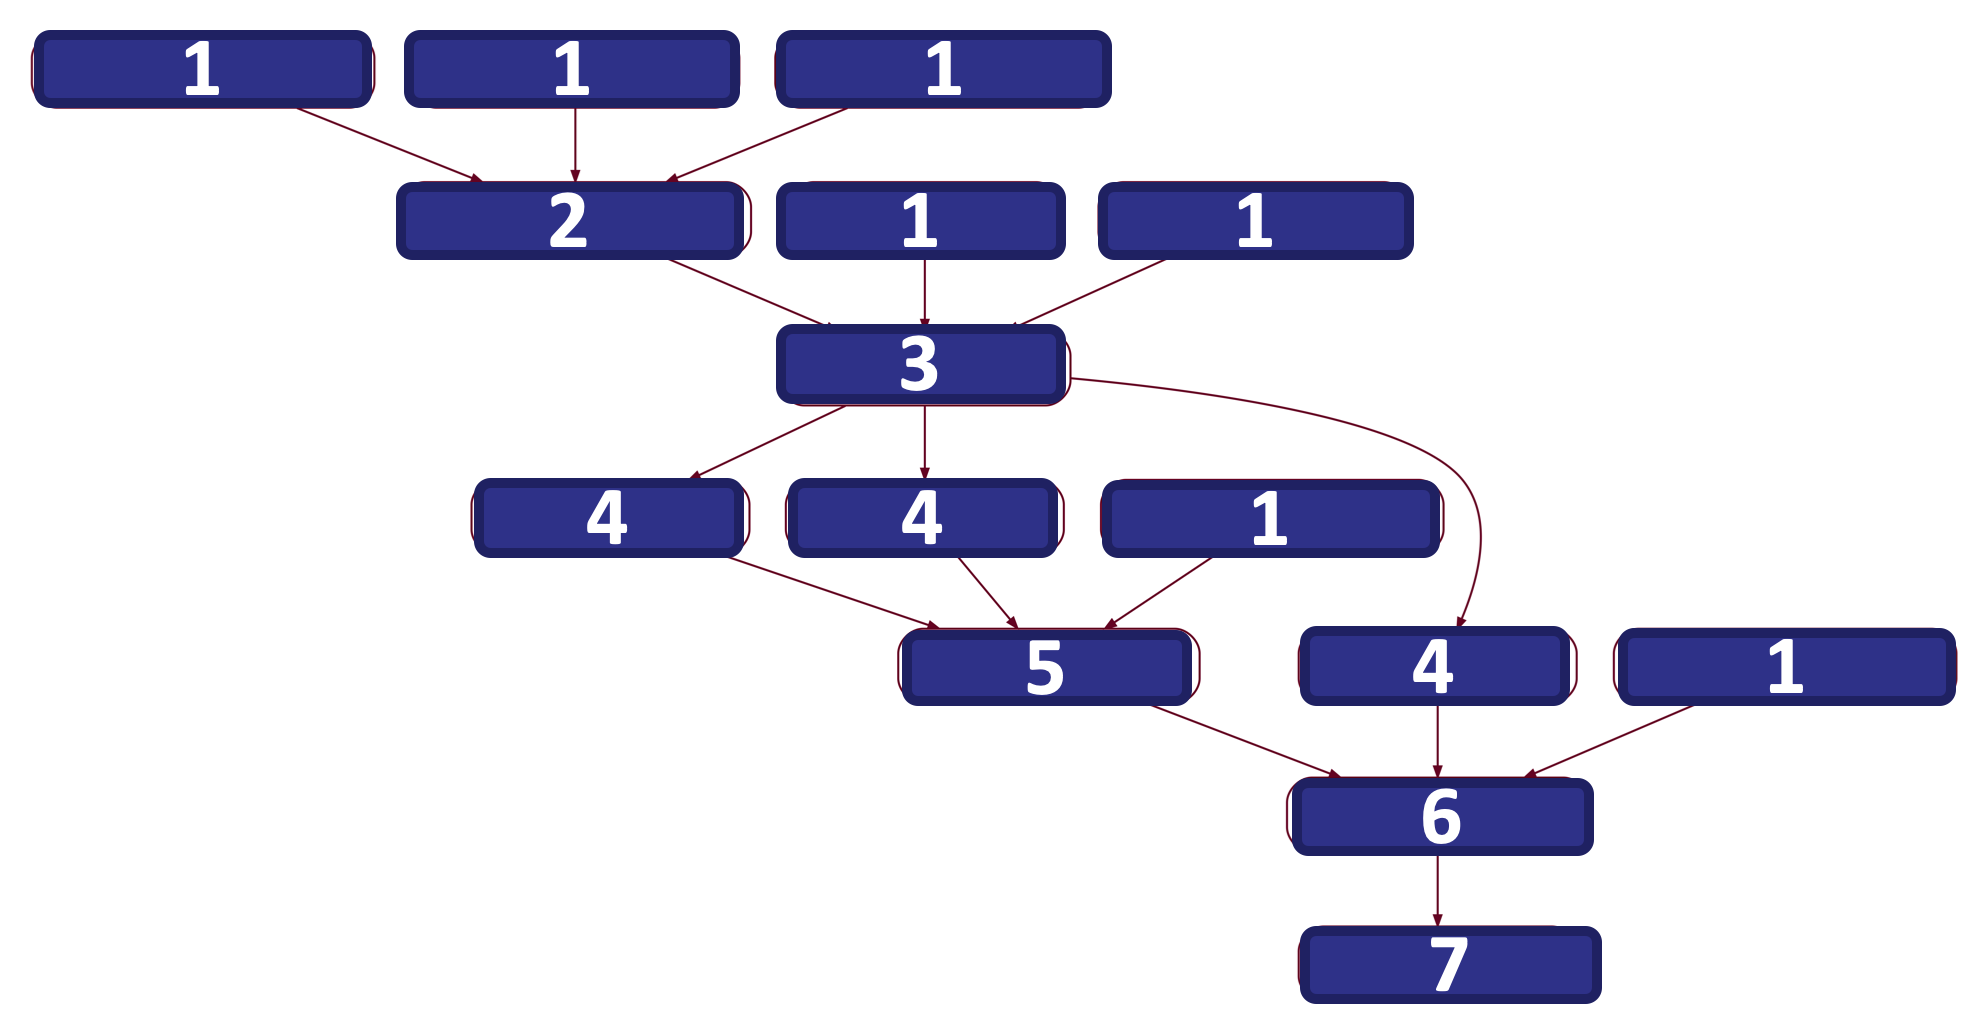
\includegraphics[width=\textwidth]{Labeled-PETPT-NFG}%
    \caption[MGD Labeled Nodes of PETPT NFG]{This figure shows the PETPT NFG with the nodes labeled according to MGD values.} \label{fig:labeled_petpt_nfg}
\end{figure}
\FloatBarrier

Adding all function nodes to the appropriate execution stack levels completes the creation of the GrFN execution stack and ensures that the GrFN can be efficiently executed.
Algorithm~\ref{alg:exec_stack_creation} shown below details the steps required to fully create a GrFN execution stack.
Starting at the greatest MGD values, a stack level is created for each unique MGD value.
After all of the function nodes for a stack level have been placed in the level, the level can be pushed onto the execution stack.
With all of the execution levels pushed onto the stack, in descending order of MGD, the execution stack can now be used to compute over a GrFN.
The execution stack for the PETPT Fortran program is shown in Figure~\ref{fig:petpt_execution_stack} below.

\begin{algorithm}
  \caption{GrFN Execution Stack Creation}
  \label{alg:exec_stack_creation}
  \begin{algorithmic}[1]
    \Procedure{CreateExecStack}{$G$} \Comment{G is a GrFN}
      \State $F \gets$ \Call{toNetworkFlowGraph}{$G$}
      \State $depth \gets $\Call{MGD}{$F$} \Comment{Annotate $F$ with MGD values}
      \State $S \gets [[~]_{1} \ldots [~]_{depth}]$ \Comment{Initialize execution stack}
      \ForAll{$n \in F$}
        \State $l \gets n.dist$
        \State \Call{push}{$n,~S[l]$} \Comment{Add $n$ to stack level $l$ in $S$}
      \EndFor
      \State \Return $S$
      \EndProcedure
  \end{algorithmic}
\end{algorithm}

\begin{figure}[!htbp]
  \centering
  \resizebox{\textwidth}{!}{
    \begin{tikzpicture}[stack/.style={rectangle split, rectangle split parts=#1,draw, anchor=center}]
      \node[stack=7, text width=15cm, align=center]  {
        \nodepart{one} \texttt{petpt\_\_condition\_\_IF\_1\_0, petpt\_\_assign\_\_albedo\_0, \\ petpt\_\_assign\_\_albedo\_1, petpt\_\_assign\_\_td\_0, \\ petpt\_\_assign\_\_slang\_0, petpt\_\_condition\_\_IF\_2\_0, \\ petpt\_\_condition\_\_IF\_2\_1}
        \nodepart{two}\texttt{petpt\_\_decision\_\_albedo\_2}
        \nodepart{three}\texttt{petpt\_\_assign\_\_eeq\_0}
        \nodepart{four}\texttt{petpt\_\_assign\_\_eo\_0, petpt\_\_assign\_\_eo\_1, \\ petpt\_\_assign\_\_eo\_2}
        \nodepart{five}\texttt{petpt\_\_decision\_\_eo\_3}
        \nodepart{six}\texttt{petpt\_\_decision\_\_eo\_4}
        \nodepart{seven}\texttt{petpt\_\_assign\_\_eo\_5}
      };
    \end{tikzpicture}
  }
  \caption[PETPT GrFN Execution Stack]{This figure shows the execution stack partial ordering for the PETPT GrFN model. The names present in the stack correspond to function nodes that are showed in PETPT's NFG diagram in Fig~\ref{fig:petpt_nfg}. Executing a stack level is accomplished by executing all of the function nodes contained in the stack level. Executing all of the stack levels illustrated here, in order, completes execution of the PETPT GrFN.}
  \label{fig:petpt_execution_stack}
\end{figure}

Algorithm~\ref{alg:stack_execution} shown below describes the detailed procedure necessary to compute the output of a GrFN from an input set.
Computing a GrFN with an execution stack is as simple as popping execution levels one at a time, executing all function nodes in the level in any order, and then repeating with the next level until no levels remain.
During execution, popped execution levels from the execution stack can be pushed onto a new stack.
After execution, the execution levels can be popped from the temporary stack and pushed back on to the original execution stack.
This ensures that the execution stack order will be maintained for the next execution.
During execution, a GrFN utilizes a value storage tag at each variable node.
When it is time to execute a function node the input data for the function node is gathered from the value tag of each parent variable node to the function node.
The output from the function node is stored in the value tag of the variable node that is the child of the function node.
After all function nodes have been executed the output variable node of the GrFN will have the computed output value stored in its value tag.

\begin{algorithm}
  \caption{Input Set Execution on GrFN}
  \label{alg:stack_execution}
  \begin{algorithmic}[1]
    \Procedure{Execute}{G, S, I} \Comment{G is a GrFN and I is an input set}
      \State \Call{setInputs}{$G,~I$} \Comment{Assign values in $I$ to $G$}
      \ForAll{$L \in S$} \Comment{Loop over each stack level in $S$}
        \ForAll{$fn \in L$} \Comment{Loop over function nodes in level $L$}
          \State $args \gets$ \Call{predecessorsOf}{$fn$}
          \State $out \gets$ \Call{successorsOf}{$fn$}
          \State $n \gets$ \Call{$fn$}{$args$} \Comment{Evaluate the function node}
          \State \Call{setNodeValue}{$out,~n,~G$}
        \EndFor
      \EndFor
      \State \Return \Call{getOutput}{$G$} \Comment{Return the value of the output node of $G$}
    \EndProcedure
  \end{algorithmic}
\end{algorithm}

\subsection{Data Type Assignment\label{sec:data_type_assg}}
So far we have introduced the wiring needed to create the computation graph that allows a GrFN to be executed, and we have described the processes necessary to make the GrFN executable.
However, one more crucial item to discuss is how GrFNs handle the actual data being processed.
Currently only basic data types are allowable in a GrFN.
This includes numerical, string, and boolean values.
The instantiations of these primitive data types are all singular values that represent a single phenomena, thus each datum matches with the definition of a variable node in GrFN.
The specification of each variable in a GrFN contains a type annotation that declares the data type of the variable.
These values are found in the descriptions of variables used in statements that are a part of the container collection sent as input to UMAF by the PA module.
During the wiring stage of UMAF, the type annotations are included in the definition of variable nodes that are added to the GrFN.
At execution time, these type annotations are used to validate a set of inputs and ensure proper storage format of computed variable values.

The infrastructure to represent complex data types such as arrays, user-defined types, and unions as part of the statements in the container collection is still being developed by the PA module team.
The main challenge with representing these data types is that they are not singular variables, but are instead collections of variables.
Collections of variables need to have accessors and setters in order to retrieve values from the collection and place values into the collection.
This presents a problem of representation that will be studied and resolved in future work.

\section{Connecting GrFN to Graphical Modeling\label{sec:grfns_are_pgms}}
The ability of GrFNs to be executed opens the door for them to also be used for model comparison and analysis.
Since GrFNs are models of observable phenomena they must be able to represent beliefs about uncertainty in the observable variables of the real-world system they represent.
Doing so allows GrFNs to be used for methods of analysis that incorporate uncertainty information about model inputs into a measure of comparative model fitness.
Domain modelers commonly use probabilistic graphical models (PGMs) during the study of observable systems to reason about the uncertainty present in the model \citep{pearl2014probabilistic}; therefore, in this section we show that GrFNs are a type of PGM.
Once it has been established that a GrFN is a PGM we show that GrFNs are members of a specific class of PGMs called Dynamic Bayesian Networks (DBNs).

All PGMs are graphs of variables of the system that they are designed to model.
These graphs encode conditional dependence amongst the nodes in the graph by linking nodes that are dependent upon one another with an edge.
PGMs whose graphs are acyclic and have directed edges are known as bayesian networks \citep{bishop2006pattern}.
By the definition of a GrFN function network given in section~\ref{sec:translation_func_net} we can see that GrFNs are closely related to bayesian networks, because they are graph-based structures that have directed edges and are defined to be acyclic.
To assert that GrFNs are indeed bayesian networks we need to show that the connections between nodes in the function network correspond to conditional dependence of child nodes upon their parents.
Due to the bipartite nature of GrFNs, paths between a set of parent variable nodes and a direct child variable are always separated by a single function node.
We can condense this representation to contain only variable nodes, where the function node computation is implied to be contained in the child variable node.
This view of the function network is known as the Causal Analysis Graph (CAG), an example of which is show in Figure~\ref{fig:petpt_cag} for the PETPT model.
CAGs depict the dependencies amongst variables in the network in the same way they would be shown in a bayesian network.
The dependencies shown also entail a conditional dependence of child nodes upon their parent nodes, due to the child node computation that contains the values of parent nodes as a component of the computation.
Therefore the directed edges of a GrFN function network do represent the conditional dependencies between the variable nodes they contain, thus GrFNs are indeed bayesian networks.

\begin{figure}[!tbp]
  \centering
  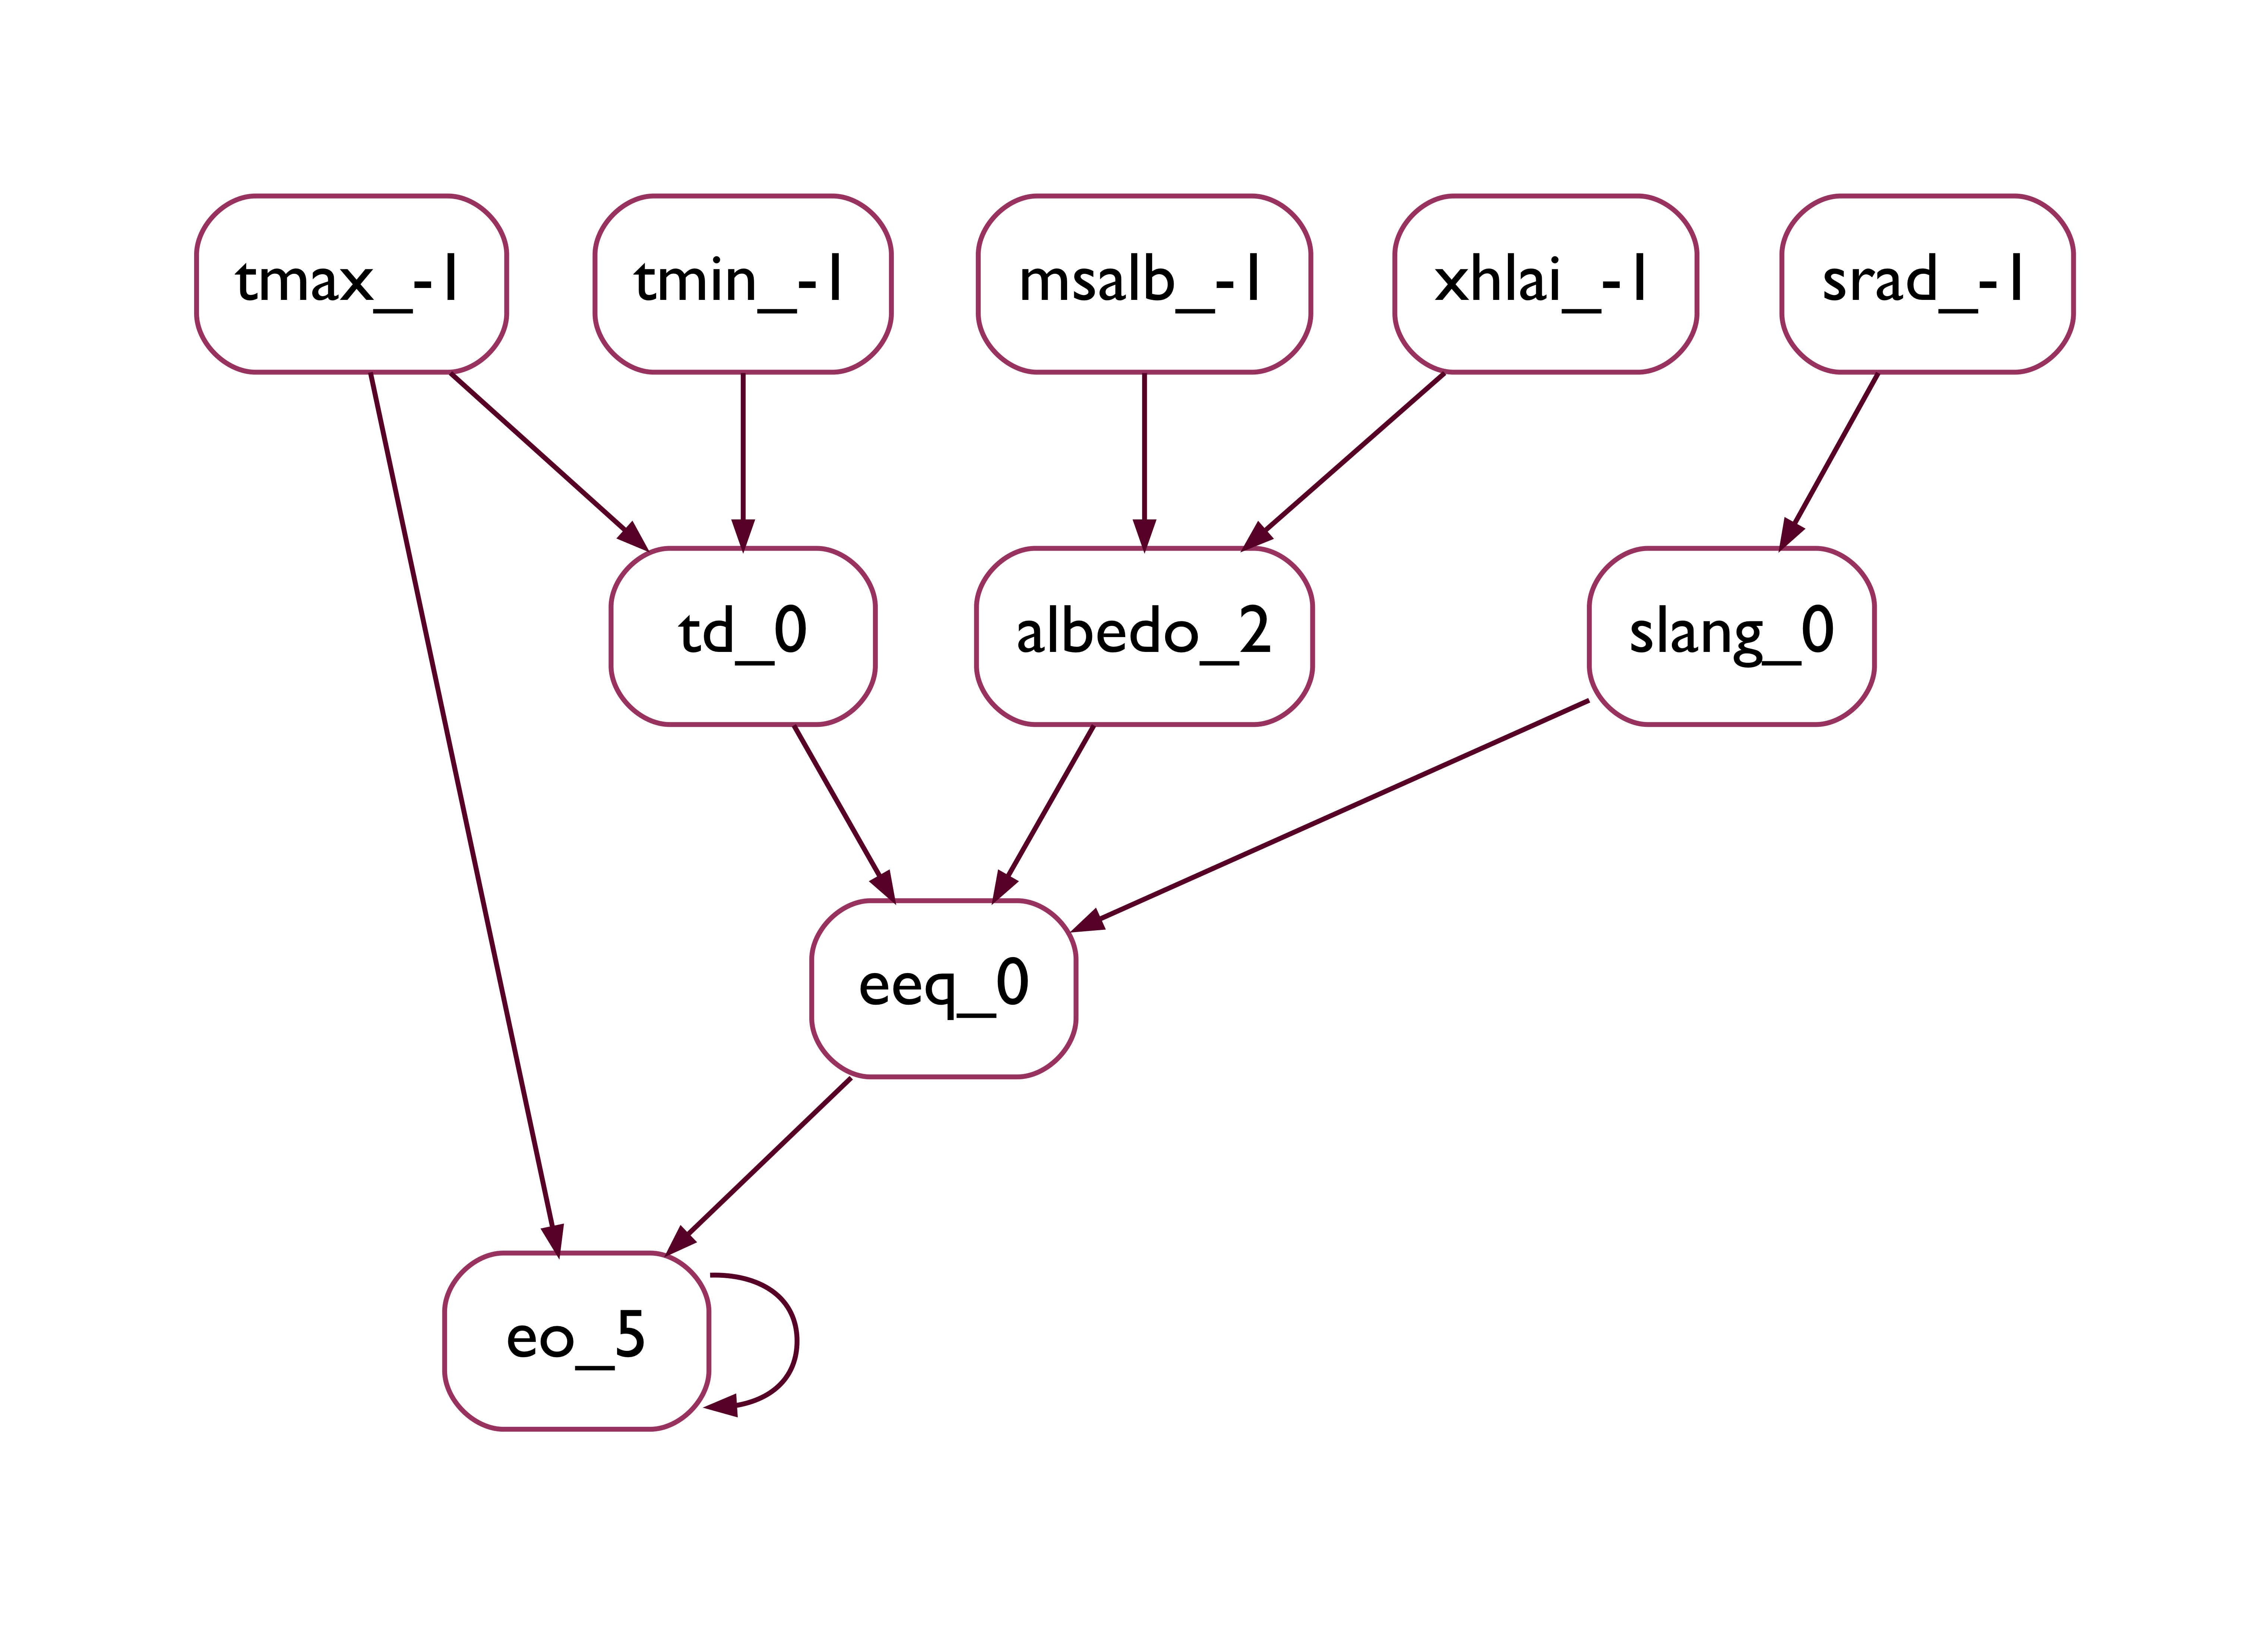
\includegraphics[width=0.8\textwidth]{PETPT_GrFN_CAG}
  \caption[PETPT GrFN Causal Analysis Graph]{An illustration of the Causal Analysis Graph (CAG) extracted from the GrFN for the PETPT evapotranspiration model.}
  \label{fig:petpt_cag}
\end{figure}

Within the class of bayesian networks exists a subclass of networks known as Dynamic Bayesian Networks (DBNs).
DBNs are characterized by being a bayesian network that has an index over the nodes in the network such that chains of related nodes are indexed to form a sequence \citep{pearl2009causality}.
This is represented in GrFN as the indexes attached to the variable name of the different variables from the original source code that track changes that occur to the variable during the course of the program.
The use of this style of indexing ensures that chains of variables in GrFN that reference the same observable real-world variable are dynamically grouped by the same indexing scheme.
This shows that not only are GrFNs a bayesian network, but that they are also DBNs.

\section{GrFN Language Feature Coverage Analyses\label{sec:grfn_eval}}
UMAF is a component of the AutoMATES pipeline, and as the AutoMATES team has been progressing, the PA module team has been able to handle more Fortran programs that can be parsed and translated into GrFNs.
In order for the pipeline process to be complete, two separate components must be able to handle the input source code program.
First the PA module must be able to parse the source code and translate its AST into the container and function collections.
Afterwards, UMAF must be able to translate the container and function collections into a GrFN that can be interpreted for execution.
Several issues can arise that require extra development in both of these components of the larger AutoMATES pipeline in order to ensure that new source code models can be translated to GrFN.
Some examples of issues that could arise would be Fortran source code constructs that have not been encountered before, or arithmetic computations that require translation to equivalent operations in the execution language of GrFN.
This section details two language feature coverage analyses on the PA module and UMAF to evaluate the coverage of our translation process from original source code to GrFN.
This section will first examine the current program idiom coverage of UMAF when translating programs to GrFNs.
The section concludes with a discussion of a selection sample study that seeks to determine how many Fortran source code models from the DSSAT code base can be parsed by the PA module and translated into GrFN.

\subsection{General Program Idiom Coverage\label{sec:supported_program_constructs}}
As discussed previously, many models that currently exist in source code are defined in imperative programming languages.
While these languages have several differences, they all share a general set of constructs that are used to define the models as source code.
To make GrFN as useful as possible to domain modelers the translation process that forms a GrFN from the imperative source code will need to be able to handle these constructs.
Not all of the constructs found in the imperative languages will need to be present in GrFN, since GrFN is a dataflow programming language.
However, all of the dataflow present in any imperative programming construct must be present in GrFN.
In Table~\ref{tab:prog_idioms} a list of imperative programming idioms is shown as well as the current GrFN coverage of the idiom.

\subsection{Fortran to GrFN Translation Evaluation\label{sec:translation_eval}}
Since the AutoMATES project is still in its early stages, GrFN does not yet cover all the programming idioms needed to guarantee coverage of any source code program, but the programming idioms that are currently covered allow for some source code models in the DSSAT codebase to be translated to GrFN.
In order to determine the extent of GrFN coverage of the DSSAT codebase a sample of $10$ Fortran programs was taken from the DSSAT codebase (in addition to the PETPT and PETASCE models being studied during the course of this thesis).
This sample of programs was sent through the AutoMATES pipeline to determine how many of the programs could be handled by the PA module and then to determine the accuracy of the GrFN translation of the programs that were parsed correctly by the PA module.
Programs that failed to be parsed by the PA module were inspected to determine which Fortran construct caused the parser to fail.
For the purpose of this study accuracy in translation to GrFN is defined by precision (P), recall (R), and F1 (F1) measures of the directed edges between variable nodes in the GrFN CAG.
P, R, and F1 are all measures defined over the interval $[0,~1]$ where higher scores represent better performance.
If additional edges between the nodes in the GrFN are seen in the CAG that do not exist in the original source code the precision score will be lower.
Equivalently, if directed edges that existed in the source code are not found in the GrFN then the recall score will be lower.
F1 is the harmonic mean of the precision and recall scores, meaning that any lowering of either of those scores will drastically lower the F1 score.
Table~\ref{tab:pa_eval_table} records the results for the sample study in terms of which Fortran files were able to be parsed and how accurate the GrFN translation was for the Fortran files that were able to be translated to GrFN.
As the results of the study indicate, the GrFN translation process was able to achieve perfect accuracy in translation for the source code programs that were able to be translated to GrFN.

\FloatBarrier
\begin{table}[!htpb]
  \centering
  \resizebox{0.8\textwidth}{!}{
    \begin{tabular}{ |c|c| }
     \hline
     \textbf{Imperative Program Idiom} & \textbf{GrFN Representation Status} \\
     \hline
     Variable Declarations & Included \\
     Assignment Statement & Included \\
     Conditional Statement & Included \\
     Procedure Calls & Included \\
     Indexed Loops & Included \\
     Open-ended Loops & In Progress \\
     Case Statements & In Progress \\
     File I/O & In Progress \\
     Array Indexing & In Progress \\
     Derived Types & In Progress \\
     Multiple/Variable Outputs & Future \\
     Early Exit & Future \\
     Error Cases & Future \\
     \hline
    \end{tabular}
  }
  \caption[GrFN Program Idiom Coverage]{Programming idiom coverage of the GrFN representation language. Note that many programming idioms may be absent from this table and others that are not normally included are present. This is due to the nature of GrFN as representing a subset of programs that are used to communicate models and needing to represent programs in the form of a graphical model for inference.}
  \label{tab:prog_idioms}
\end{table}

\begin{table}
  \centering
  \resizebox{\textwidth}{!}{
    \begin{tabular}{ |c|c|c|l| }
      \hline
      \textbf{Model Identifier} & \textbf{Parse Status} & \textbf{P,R,F1 Scores} & \textbf{Cause of Failure} \\
      \hline
      PETPT & \cmark & 1.0, 1.0, 1.0 & -- \\
      PETASCE & \cmark & 1.0, 1.0, 1.0 & -- \\
      \hline
      FLOOD\_EVAP & \cmark & 1.0, 1.0, 1.0 & -- \\
      SOLAR & \cmark & 1.0, 1.0, 1.0 & -- \\
      DECL & \xmark & -- & User-defined functions \\
      INSOIL & \xmark & -- & Unknown builtin functions \\
      PETPEN & \xmark & -- & Assignment before declaration \\
      ROOTWU & \xmark & -- & Variable range iteration \\
      MULCH\_EVAP & \xmark & -- & Use of derived types \\
      SNOWFALL & \xmark & -- & Nested if-statements \\
      EFLOW\_C & \xmark & -- & Early conditional exit \\
      ESUP & \xmark & -- & Multiple/variable outputs \\
      \hline
    \end{tabular}
  }
  \caption[Program Analysis Module Evaluation]{Evaluation results for the program analysis module. This evaluation tested the program analysis modules capability to parse and transfer correct GrFN representation wiring for 10 models found in the DSSAT Fortran codebase.}
  \label{tab:pa_eval_table}
\end{table}
\FloatBarrier
